\documentclass[12pt,a4paper]{report}

% --- Codificación e idioma ---
\usepackage[utf8]{inputenc}
\usepackage[T1]{fontenc}
\usepackage[spanish,es-tabla,es-nodecimaldot]{babel}
\usepackage{mathptmx} % Times New Roman para texto y matemáticas

% --- Matemáticas y tablas ---
\usepackage{amsmath,amssymb}
\usepackage{array}
\usepackage{booktabs}
\usepackage{tabularx}
\usepackage{multirow}

% --- Gráficos, código y color ---
\usepackage{graphicx}
\graphicspath{{figures/}}
\usepackage{listings}
\usepackage{xcolor}
\usepackage{caption}

% --- Geometría e interlineado (formato memoria UNIE) ---
\usepackage{geometry}
\geometry{a4paper,top=2.5cm,bottom=2.5cm,left=3cm,right=2.5cm}
\usepackage{setspace}
\onehalfspacing

% --- Bibliografía APA (autor-año) con apacite + bibtex, localización ES ---
% (alternativa a biblatex/biber: biber no es compatible con la versión de
%  biblatex incluida en el compilador; apacite usa bibtex y localiza con babel.)
% apacite se carga ANTES de hyperref para evitar el conflicto \@year@.
\usepackage[natbibapa]{apacite}   % compatibilidad natbib (convive con hyperref)
\let\textcite\citet   % autor (año)
\let\parencite\citep  % (autor, año)
\renewcommand{\bibname}{Referencias}

\usepackage[hidelinks]{hyperref}
\usepackage{enumitem}
\usepackage{tikz}
\usetikzlibrary{shapes.geometric,arrows.meta,positioning}
\usepackage{pgfplots}
\pgfplotsset{compat=1.18}

\setlength{\parskip}{0.6\baselineskip}
\renewcommand{\contentsname}{Índice general}

% --- Estilo de listados de código/terminal ---
\definecolor{codebg}{RGB}{28,28,28}
\definecolor{codefg}{RGB}{235,235,235}
\definecolor{kwcolor}{RGB}{120,170,255}
\lstdefinestyle{terminal}{
  basicstyle=\ttfamily\footnotesize\color{codefg},
  backgroundcolor=\color{codebg},
  frame=single,
  framerule=0pt,
  rulecolor=\color{codebg},
  xleftmargin=4pt,
  xrightmargin=4pt,
  aboveskip=0.8\baselineskip,
  belowskip=0.5\baselineskip,
  columns=fullflexible,
  keepspaces=true,
  breaklines=true,
  showstringspaces=false,
  inputencoding=utf8,
  extendedchars=true,
  literate=
    {á}{{\'a}}1 {é}{{\'e}}1 {í}{{\'i}}1 {ó}{{\'o}}1 {ú}{{\'u}}1
    {Á}{{\'A}}1 {É}{{\'E}}1 {Í}{{\'I}}1 {Ó}{{\'O}}1 {Ú}{{\'U}}1
    {ñ}{{\~n}}1 {Ñ}{{\~N}}1 {ü}{{\"u}}1 {Ü}{{\"U}}1
    {¿}{{?`}}1 {¡}{{!`}}1 {ρ}{{$\rho$}}1 {≈}{{$\approx$}}1
}
\lstdefinestyle{pycode}{
  style=terminal,
  backgroundcolor=\color{white},
  basicstyle=\ttfamily\footnotesize\color{black},
  frame=single,
  rulecolor=\color{black!30},
}

\begin{document}

% ======================= PORTADA =======================
\begin{titlepage}
  \centering
  \vspace*{1cm}
  {\scshape\large Universidad UNIE\par}
  {\scshape Grado en Ingeniería Informática\par}
  \vspace{2.2cm}
  {\Large\bfseries Trabajo de Fin de Grado\par}
  \vspace{1.2cm}
  \rule{\linewidth}{0.4pt}\par\vspace{0.5cm}
  {\LARGE\bfseries Sistema automático de corrección de preguntas abiertas a partir de imágenes de exámenes\par}
  \vspace{0.5cm}
  \rule{\linewidth}{0.4pt}\par
  \vspace{2.2cm}
  \begin{flushright}
    \begin{tabular}{rl}
      \textbf{Autor:} & Adrián Soler Rodríguez\\[0.3cm]
      \textbf{Tutor:} & Beatriz Magán Pinto\\[0.3cm]
      \textbf{Curso académico:} & 2025--2026\\[0.3cm]
      \textbf{Convocatoria:} & Extraordinaria\\
    \end{tabular}
  \end{flushright}
  \vfill
  {\large Madrid, 2026\par}
\end{titlepage}

\pagenumbering{roman}
\setcounter{page}{2}

\chapter*{Resumen}
\addcontentsline{toc}{chapter}{Resumen}

La corrección de preguntas abiertas es una de las tareas más costosas de la evaluación académica, porque obliga a interpretar texto libre y a distinguir entre respuestas correctas, parciales y conceptualmente erróneas. Este trabajo presenta el diseño y desarrollo de un sistema automático que corrige este tipo de preguntas a partir de imágenes de exámenes, organizado como un \emph{pipeline} que integra reconocimiento óptico de caracteres, separación de pregunta y respuesta, una respuesta de referencia y un módulo de evaluación semántica que combina conceptos clave ponderados, similitud global y control de longitud.

El núcleo del sistema es deliberadamente determinista e interpretable: la nota se puede justificar señalando qué conceptos aparecen, cuáles faltan y por qué. Sobre esa base se han incorporado cuatro mejoras que responden a limitaciones observadas durante las pruebas: un análisis de polaridad que evita acreditar conceptos negados o mal atribuidos, sinónimos por concepto que reconocen paráfrasis válidas, un verificador de factualidad opcional basado en un modelo de lenguaje que actúa como segunda opinión sin reescribir la nota, y una capa de calibración que ajusta la escala del sistema al criterio de cada corrector.

La validación no se limita a casos aislados. Se ha construido una batería de prueba determinista, un banco de exámenes conceptuales que cubre desde Primaria hasta Máster, y una validación con datos reales corregidos por profesores (el conjunto de Mohler). Sobre el banco propio, el sistema concuerda con la calificación de referencia con una correlación de Spearman de $\rho \approx 0{,}93$ y un error medio inferior a un punto sobre diez; sobre datos externos en inglés y sin rúbrica curada, el rendimiento desciende a $\rho \approx 0{,}54$, y se demuestra que ese desfase es sobre todo de escala y se corrige con la capa de calibración. Estos resultados delimitan con números cuándo el corrector es fiable y cuándo necesita la intervención del profesor.

\vspace{0.8cm}
\noindent\textbf{Palabras clave:} corrección automática, preguntas abiertas, evaluación semántica, OCR, conceptos clave, correlación de Spearman, calibración, interpretabilidad.

\chapter*{Abstract}
\addcontentsline{toc}{chapter}{Abstract}

Grading open-ended questions is one of the most time-consuming tasks in academic assessment, since it requires interpreting free text and telling apart correct, partial and conceptually wrong answers. This project presents the design and development of an automatic system that grades such questions from exam images, structured as a pipeline that integrates optical character recognition, question–answer separation, a reference answer and a semantic evaluation module combining weighted key concepts, global similarity and a length control.

The core of the system is deliberately deterministic and interpretable: every grade can be justified by stating which concepts are present, which are missing and why. On top of that core, four improvements address limitations observed during testing: a polarity analysis that prevents crediting negated or misattributed concepts; per-concept synonyms that recognise valid paraphrases; an optional large-language-model factuality verifier that acts as a second opinion without overwriting the grade; and a calibration layer that adjusts the system scale to each grader's criterion.

Validation goes beyond isolated cases. A deterministic test suite, a bank of conceptual exams spanning from primary school to a master's degree, and a validation against real teacher-graded data (the Mohler dataset) were built. On the in-house bank the system agrees with the reference grade with a Spearman correlation of $\rho \approx 0.93$ and a mean error below one point out of ten; on external English data without a curated rubric, performance drops to $\rho \approx 0.54$, and this gap is shown to be mostly a matter of scale, which the calibration layer corrects. These results quantify when the grader is reliable and when it still needs the teacher.

\vspace{0.8cm}
\noindent\textbf{Keywords:} automatic grading, open-ended questions, semantic evaluation, OCR, key concepts, Spearman correlation, calibration, interpretability.

\clearpage


\tableofcontents
\clearpage

\pagenumbering{arabic}
\setcounter{page}{1}

\chapter{Introducción y objetivos}

\section{Introducción}

La corrección de preguntas abiertas sigue siendo una de las tareas más costosas dentro de la evaluación académica. A diferencia de los test cerrados, este tipo de ejercicios exige interpretar texto libre, valorar si el contenido responde realmente a lo planteado y, en muchos casos, distinguir entre respuestas incompletas, parcialmente correctas o conceptualmente erróneas. Cuando además la respuesta del alumno se entrega en formato manuscrito o escaneado, el problema incorpora una etapa previa de extracción de información que condiciona todo el proceso posterior.

Este trabajo aborda el diseño y desarrollo de un sistema automático de corrección de preguntas abiertas a partir de imágenes de exámenes. El objetivo no es resolver únicamente la lectura óptica de caracteres ni limitarse a una comparación superficial entre cadenas de texto, sino construir un flujo de evaluación completo capaz de transformar una imagen de entrada en una calificación razonada acompañada de retroalimentación. Para ello se plantea una arquitectura en \emph{pipeline} en la que cada fase cumple una función específica: preprocesamiento de imagen, OCR, identificación de la pregunta y la respuesta, generación de una respuesta ideal de referencia, evaluación semántica y producción de una nota final.

La parte central del sistema reside en la evaluación semántica. En un contexto de respuesta abierta, comparar únicamente palabras o expresiones literales resulta insuficiente, ya que dos alumnos pueden expresar una misma idea con distinta redacción, diferente orden sintáctico o niveles desiguales de detalle. Por ese motivo, la solución propuesta combina varios criterios: detección de conceptos clave ponderados, medida de similitud global del texto y penalización por longitud cuando la respuesta se desvía de forma significativa respecto a lo esperable. Esta combinación permite obtener una valoración más equilibrada que la que se lograría con un enfoque basado solo en coincidencias exactas.

Este trabajo no implementa un modelo de aprendizaje automático entrenado sobre datos, sino un sistema de evaluación diseñado mediante reglas y heurísticas semánticas. Esa decisión es intencionada: en un contexto evaluativo, poder explicar por qué una respuesta ha recibido una determinada nota es tan importante como la nota misma. Aun así, el sistema incorpora elementos propios de la inteligencia artificial, como la interpretación del lenguaje mediante conceptos clave, la aproximación a la evaluación humana y, en una capa opcional y claramente acotada, el uso de un modelo de lenguaje como segunda opinión. Por ello puede clasificarse como un sistema automático híbrido, con un núcleo basado en reglas y componentes opcionales de inteligencia artificial.

El sistema desarrollado tiene un enfoque aplicado y realista. No pretende sustituir completamente la corrección humana en cualquier escenario, sino ofrecer una base técnica útil para automatizar parte del proceso en contextos acotados, especialmente cuando las preguntas pertenecen a dominios bien definidos y existe una estructura mínima en los criterios de evaluación. Desde esa perspectiva, el trabajo se sitúa entre la visión experimental y la implementación de una herramienta práctica de apoyo a la docencia.

Conviene señalar desde el principio que la versión aquí descrita es el resultado de varias iteraciones. El proyecto partió de un \emph{pipeline} de OCR y evaluación por conceptos, y fue creciendo a medida que las pruebas revelaban comportamientos no deseados. Buena parte de lo que en una primera memoria figuraba como ``trabajo futuro'' —reconocer paráfrasis, detectar respuestas que niegan lo correcto, validar contra notas humanas reales o medir la correlación con un corrector— se ha terminado implementando y se documenta aquí ya como resultado, no como propósito.

\section{Motivación}

La motivación principal de este trabajo surge de una necesidad muy concreta: reducir el tiempo invertido en la corrección manual de preguntas abiertas sin perder completamente la capacidad de valorar el contenido de la respuesta. En entornos educativos con grupos numerosos, la revisión de exámenes con desarrollo corto o medio supone una carga relevante para el profesorado, especialmente cuando se busca mantener criterios homogéneos entre distintos alumnos.

En la práctica, muchas soluciones de corrección automática se han centrado históricamente en preguntas tipo test o en ejercicios con respuesta muy estructurada. Sin embargo, las preguntas abiertas siguen teniendo un papel importante porque permiten comprobar comprensión, capacidad de síntesis y uso adecuado de conceptos. Precisamente por eso son valiosas desde el punto de vista docente, aunque también resulten más difíciles de automatizar.

Otro factor que refuerza la relevancia del proyecto es que, en numerosos contextos, las respuestas no se reciben como texto digital nativo, sino como imágenes generadas a partir de escaneos, fotografías o documentos exportados desde plataformas de examen. Esto añade una dificultad adicional: antes de evaluar la calidad de la respuesta es necesario extraerla de forma razonablemente fiable. Por tanto, el problema no puede abordarse solo desde el procesamiento del lenguaje natural, sino como una integración entre visión por computador, OCR y análisis semántico.

Además del interés académico, el proyecto tiene valor desde una perspectiva de ingeniería. Obliga a conectar varios módulos heterogéneos, a tomar decisiones sobre cómo representar el conocimiento relevante de una pregunta y a definir una métrica de evaluación interpretable. En lugar de confiar en una única puntuación opaca, se ha buscado que el sistema pueda justificar el resultado mediante criterios comprensibles, como la presencia de conceptos esperados o el grado de proximidad global entre la respuesta del alumno y una respuesta modelo.

\section{Objetivo general}

El objetivo general del trabajo es desarrollar un sistema automático capaz de corregir preguntas abiertas a partir de imágenes de exámenes, generando una nota y una retroalimentación básica de forma coherente con unos criterios de evaluación predefinidos, y hacerlo de manera que el resultado sea interpretable y defendible ante un corrector humano.

\section{Objetivos específicos}

Para alcanzar ese objetivo general se plantean los siguientes objetivos específicos:

\begin{itemize}[leftmargin=1.4em]
  \item Diseñar una arquitectura modular que separe claramente las fases de adquisición, extracción y evaluación.
  \item Estudiar el pretratamiento de imagen previo al OCR y evaluar empíricamente su impacto real sobre la calidad de la extracción.
  \item Integrar Tesseract como motor de reconocimiento óptico de caracteres para convertir la imagen en texto procesable.
  \item Identificar dentro del texto extraído los fragmentos correspondientes a la pregunta y a la respuesta.
  \item Generar una respuesta ideal o de referencia que actúe como base para la comparación posterior.
  \item Definir un mecanismo de evaluación semántica que combine conceptos clave ponderados, similitud global y control de longitud.
  \item Dotar al sistema de robustez frente a dos fallos típicos de la corrección por palabras clave: las respuestas que niegan lo correcto y las que reutilizan el vocabulario del tema sin comprenderlo.
  \item Reconocer paráfrasis válidas mediante sinónimos asociados a cada concepto, sin renunciar a la interpretabilidad.
  \item Validar el sistema de forma cuantitativa, midiendo su concordancia con notas humanas tanto de referencia como reales, mediante correlación de Spearman y error medio.
  \item Analizar las limitaciones reales del sistema y proponer mejoras viables para futuras iteraciones.
\end{itemize}

\section{Alcance del proyecto}

El alcance del sistema se ha acotado deliberadamente para mantener una relación razonable entre complejidad y viabilidad. La propuesta se orienta a preguntas abiertas de extensión limitada o media, pertenecientes a dominios donde sea posible definir conceptos relevantes con cierta claridad. No se ha planteado como una solución universal para cualquier disciplina, ni como un sustituto completo del criterio docente.

Tampoco se persigue resolver todos los problemas asociados al reconocimiento de escritura manuscrita compleja o a imágenes de baja calidad extrema. El foco del trabajo está en demostrar que, bajo unas condiciones de entrada razonables, es posible construir un \emph{pipeline} completo de corrección automática que produzca resultados útiles y defendibles. Esta delimitación permite centrar el esfuerzo en la lógica del sistema y, en particular, en el diseño de la evaluación semántica.

Conviene precisar también qué tipos de pregunta entran en el alcance del módulo principal. El corrector semántico está pensado para preguntas conceptuales: definiciones, explicaciones y enunciados teóricos en los que la respuesta correcta se puede describir mediante un conjunto de ideas clave. Las preguntas de cálculo numérico y las de redacción libre (comentario de texto, expresión en lengua extranjera) quedan fuera de ese módulo y se atienden, cuando procede, con componentes específicos que se describen más adelante. Reconocer esa frontera es parte del trabajo: un sistema honesto debe saber qué preguntas puede juzgar bien y cuáles conviene derivar a otro mecanismo.

\section{Principales contribuciones}

Aunque el objetivo general es construir un sistema funcional, conviene destacar las aportaciones concretas que diferencian este trabajo de un simple ensamblaje de herramientas:

\begin{itemize}[leftmargin=1.4em]
  \item Un corrector semántico determinista e interpretable que combina conceptos clave ponderados, similitud global y control de longitud, con una fórmula de nota cuyo orden de operaciones está justificado.
  \item Un análisis de polaridad que evita el fallo más grave de la corrección por palabras clave —puntuar alto una respuesta que niega lo correcto— manteniendo la trazabilidad.
  \item Un mecanismo de sinónimos por concepto que reconoce paráfrasis sin perder interpretabilidad y sin alterar el comportamiento previo del sistema.
  \item Una capa de verificación opcional que detecta atribuciones erróneas como segunda opinión, sin reescribir la nota.
  \item Una capa de calibración determinista que ajusta la escala del sistema a la de un corrector concreto, validada sobre datos no vistos.
  \item Una validación cuantitativa amplia: una batería determinista, un banco de exámenes de cinco niveles educativos y una prueba con notas de profesores humanos reales, con resultados expresados mediante correlación de Spearman y error medio.
\end{itemize}

\section{Estructura de la memoria}

El resto del documento se organiza como sigue. El capítulo~\ref{cap:estado} revisa el estado del arte en corrección automática de respuestas abiertas, OCR en documentos académicos y evaluación semántica, y justifica el enfoque adoptado. El capítulo~\ref{cap:metodologia} describe la metodología y el desarrollo: la arquitectura del \emph{pipeline}, cada uno de sus módulos y las mejoras incorporadas (polaridad, sinónimos, verificador y calibración), así como la aplicación web construida para la demostración. El capítulo~\ref{cap:resultados} recoge la validación experimental, desde la batería determinista hasta la validación con datos reales y la recalibración. El capítulo~\ref{cap:consideraciones} aborda las consideraciones éticas, legales y de sostenibilidad del sistema. El capítulo~\ref{cap:conclusiones} resume las conclusiones y las líneas de trabajo futuro. Finalmente se incluyen los anexos y las referencias.

\chapter{Estado del arte}
\label{cap:estado}

\section{Corrección automática de respuestas abiertas}

La corrección automática de texto libre, conocida en la literatura como \emph{Automatic Short Answer Grading} (ASAG), es un problema abordado desde distintos enfoques \parencite{burrows2015}. Los sistemas más simples se basan en reglas, listas de palabras clave o expresiones regulares. Su principal ventaja es la facilidad de implementación y la interpretabilidad, ya que permiten justificar la nota en función de elementos observables. Sin embargo, presentan una limitación evidente: penalizan en exceso la variabilidad lingüística. Cuando un estudiante expresa una idea correcta utilizando sinónimos, reformulaciones o una estructura distinta de la esperada, estos sistemas pueden infravalorar la respuesta.

En el extremo opuesto se sitúan métodos basados en modelos estadísticos o en representaciones semánticas densas. La aparición de los \emph{word embeddings} \parencite{mikolov2013} y, más tarde, de los modelos basados en \emph{transformers} permitió capturar significado más allá de la coincidencia literal, situando cerca, en un espacio vectorial, palabras o frases de sentido parecido. Estos enfoques son especialmente útiles cuando la diversidad de redacción es elevada. El inconveniente es que suelen requerir más datos, más capacidad de ajuste y, en ocasiones, sacrifican interpretabilidad. En entornos académicos, la posibilidad de explicar por qué una respuesta ha recibido una determinada calificación sigue siendo un requisito importante, y no siempre es compatible con un modelo cuya decisión es difícil de auditar.

Más recientemente, el uso de grandes modelos de lenguaje como evaluadores —el paradigma del \emph{LLM-as-a-judge} \parencite{zheng2023}— ha mostrado resultados notables, ya que estos modelos pueden valorar una respuesta a partir de una rúbrica expresada en lenguaje natural. No obstante, plantean dos problemas para un uso evaluativo serio: su salida no es plenamente reproducible y su razonamiento no es del todo transparente. Por ello, en este trabajo el modelo de lenguaje no se utiliza como juez principal, sino como una segunda opinión acotada y opcional, manteniendo el núcleo determinista.

En la práctica, este tipo de soluciones no siempre funcionan tan bien como se describe en teoría, especialmente cuando las respuestas son muy breves o poco estructuradas. Por ello, muchos sistemas útiles en escenarios docentes combinan distintas señales en lugar de depender de una única métrica.

\section{Conjuntos de datos de referencia}

Un aspecto recurrente en la investigación sobre ASAG es la dificultad de disponer de respuestas reales de alumnos corregidas por profesores. Existen, sin embargo, varios conjuntos de datos que sí incluyen esa información y que se han convertido en referencia para comparar sistemas.

El conjunto de \textcite{mohler2011} recoge respuestas de estudiantes de un curso universitario de informática, con alrededor de 2.400 respuestas a 87 preguntas, cada una calificada por dos correctores humanos en una escala de 0 a 5. Es especialmente valioso porque proporciona, junto a cada pregunta, una respuesta de referencia del profesor. El conjunto ASAP-SAS, difundido a través de una competición pública, ofrece un volumen mayor (en torno a 17.000 respuestas) sobre temas de ciencias a nivel escolar. Por su parte, la tarea 7 de SemEval-2013 \parencite{dzikovska2013} reúne casi 10.000 respuestas en quince dominios científicos, etiquetadas no solo con una nota sino con categorías de corrección.

Estos conjuntos comparten una limitación para el caso español: están redactados en inglés y, en su mayoría, pertenecen a dominios técnicos. Los exámenes oficiales en español que sí son públicos —por ejemplo, las pruebas de acceso a la universidad— suelen distribuir el enunciado, los criterios de corrección y una solución modelo, pero rara vez incluyen respuestas reales de alumnos con su nota, que es justamente lo que se necesita para medir la concordancia con un corrector. Esta asimetría se ha tenido en cuenta al diseñar la validación de este trabajo, que combina un banco propio en español con una prueba sobre datos reales en inglés.

\section{OCR en documentos académicos}

El reconocimiento óptico de caracteres constituye una etapa clave cuando el texto que se desea evaluar no se encuentra en formato digital nativo. Su función es transformar una imagen en una representación textual susceptible de ser procesada posteriormente. Aunque la idea general es sencilla, el rendimiento del OCR depende fuertemente de la calidad de la imagen. En documentos académicos escaneados pueden aparecer problemas como sombras, inclinación, ruido, contraste deficiente o variaciones en el tamaño de letra. Además, en el caso de respuestas escritas a mano o con formatos poco uniformes, la extracción se vuelve más inestable.

Tesseract \parencite{smith2007} es una de las herramientas más extendidas en este ámbito por su madurez, disponibilidad y capacidad para integrarse en \emph{pipelines} personalizados. En la literatura se asume con frecuencia que su rendimiento mejora cuando la imagen ha sido preprocesada de forma adecuada: convertir a escala de grises, binarizar, eliminar ruido o reforzar el contraste suelen presentarse como pasos que influyen en la calidad del texto extraído. No obstante, el beneficio real de cada una de estas operaciones depende del tipo de imagen y no puede darse por supuesto, por lo que conviene validarlo de forma empírica sobre los datos concretos del problema. Como se verá, en este proyecto esa validación llevó a una conclusión contraria a la intuición habitual.

Por tanto, en un sistema como el planteado, el OCR no puede considerarse un módulo aislado. Su salida afecta a todas las fases siguientes: un error de lectura puede alterar una palabra clave, fragmentar una frase o incluso desestructurar la separación entre pregunta y respuesta. Esto obliga a estudiar con cuidado qué tratamiento de imagen conviene aplicar antes de la extracción, valorando su efecto real sobre la lectura en lugar de asumir que cualquier preprocesamiento mejora el resultado.

\subsection{Texto manuscrito frente a texto impreso}

No es lo mismo reconocer texto impreso que manuscrito. El texto impreso presenta formas de letra regulares y un espaciado uniforme, lo que permite a un motor como Tesseract alcanzar precisiones altas con poco esfuerzo. La escritura manuscrita, en cambio, introduce una variabilidad enorme: cada persona traza las letras de forma distinta, las une de maneras diferentes y mantiene espaciados irregulares. A esto se añaden, en un examen real, las tachaduras, las correcciones, las flechas y las anotaciones al margen. Por eso el reconocimiento de manuscrito suele requerir modelos específicos, y su fiabilidad sigue siendo notablemente inferior a la del impreso.

Esta diferencia condiciona el alcance del proyecto. El sistema se ha diseñado y probado fundamentalmente sobre texto claro, asumiendo que la calidad de la entrada es razonable. Reconocer manuscrito complejo de forma fiable es un problema en sí mismo, ajeno al núcleo de este trabajo, que es la evaluación de la respuesta una vez extraída. Aun así, la robustez del módulo semántico frente a pequeños errores de lectura —mediante la detección parcial y la tolerancia a variaciones— amortigua parte de la imperfección del OCR, sin pretender resolverla por completo.

\section{Evaluación semántica y limitaciones de la comparación literal}

La comparación exacta de palabras es útil como señal inicial, pero insuficiente como criterio único de corrección. Existen varias razones para ello. En primer lugar, el lenguaje natural admite múltiples formulaciones equivalentes: una respuesta puede ser conceptualmente correcta aunque no reutilice los términos exactos del enunciado o de la solución modelo. En segundo lugar, la presencia de ciertas palabras no garantiza que el alumno haya entendido la idea; puede haber coincidencia léxica sin coherencia real, e incluso lo contrario, una negación que invierte el sentido. En tercer lugar, las respuestas abiertas suelen admitir distintos niveles de detalle, y la relevancia de cada fragmento no es homogénea.

La evaluación semántica trata precisamente de superar estas limitaciones. En términos generales, busca aproximar el significado global de un texto y valorar si contiene la información relevante desde el punto de vista conceptual. En aplicaciones reales esto suele resolverse combinando criterios locales y globales: por un lado, comprobar si aparecen elementos esenciales; por otro, medir si la respuesta, en conjunto, se parece a una referencia válida.

Un punto poco tratado en los sistemas más simples, pero crítico en evaluación, es la \emph{polaridad}. Un detector de palabras clave que solo comprueba presencia no distingue entre ``la mitocondria produce ATP'' y ``la mitocondria no produce ATP'': ambas contienen los mismos términos. La detección de la negación es un problema clásico del procesamiento del lenguaje natural, y su alcance —hasta dónde se extiende el efecto de un ``no'' dentro de una frase— condiciona la fiabilidad de cualquier corrector basado en conceptos. Este trabajo aborda explícitamente esa cuestión.

\subsection{Comparación entre enfoques de corrección}

Durante el diseño del sistema se consideraron tres estrategias principales de evaluación: comparación literal de palabras, similitud global del texto y enfoque híbrido. La diferencia entre ellas no es solo de complejidad, sino de comportamiento ante casos reales. En preguntas abiertas cortas, la elección del enfoque condiciona directamente qué errores se cometen y qué tipo de respuestas se valoran de forma injusta.

La comparación literal de palabras es el enfoque más simple. Consiste en verificar si la respuesta del alumno contiene exactamente los términos esperados. Su principal ventaja es la interpretabilidad inmediata: resulta sencillo justificar que una palabra clave aparece o no, y su implementación es poco costosa. También funciona razonablemente bien en preguntas muy cerradas. Sin embargo, su limitación es importante. Si un alumno responde correctamente usando sinónimos o reformulaciones, el sistema puede no reconocer la validez de la respuesta. Y, al revés, una frase incorrecta como ``la mitocondria es el núcleo de la célula'' contiene un término del dominio, pero eso no implica comprensión válida.

La similitud global del texto intenta corregir parte de ese problema al comparar la respuesta del alumno con una referencia completa. Su ventaja principal es que tolera mejor ciertos cambios de orden, estilo o formulación. No obstante, también presenta limitaciones claras. Puede penalizar respuestas correctas pero breves, porque la distancia con una referencia más desarrollada aumenta aunque el contenido esencial esté presente; puede verse afectada por errores de OCR que alteran varias palabras; y puede sobrevalorar respuestas superficialmente parecidas a la referencia aunque omitan un concepto esencial.

El enfoque híbrido utilizado en este proyecto combina lo más útil de ambos planteamientos y añade un control explícito sobre la longitud. La mayor parte de la nota depende de conceptos clave ponderados, mientras que la similitud global actúa solo como apoyo contextual. De esta forma el sistema mantiene interpretabilidad y, al mismo tiempo, gana tolerancia ante reformulaciones válidas. Si el alumno utiliza sinónimos o una redacción distinta, el bloque conceptual puede seguir detectando la evidencia relevante y la similitud aporta una corrección moderada. A la vez, si una respuesta reutiliza palabras del tema pero establece relaciones incorrectas, la mera coincidencia léxica no basta para obtener una puntuación alta.

En consecuencia, el enfoque híbrido resulta más adecuado para este proyecto porque se ajusta mejor a las condiciones reales del problema: respuestas abiertas, entrada afectada por OCR y necesidad de justificar la nota de forma comprensible. No es el enfoque más simple, pero sí el que ofrece un mejor equilibrio entre robustez, interpretabilidad y capacidad para distinguir entre respuestas completas, parciales e incorrectas.

\section{Herramientas y plataformas existentes}

En el ámbito comercial y académico existen plataformas que abordan partes del problema. Los sistemas de gestión del aprendizaje más extendidos incorporan corrección automática de cuestionarios, pero casi siempre limitada a preguntas de tipo test, emparejamiento o respuesta corta con solución exacta; las preguntas de desarrollo se siguen corrigiendo a mano. Existen también servicios especializados en evaluación de ensayos —el llamado \emph{automated essay scoring}— que puntúan redacciones extensas, habitualmente entrenados sobre grandes colecciones de textos calificados y orientados al inglés; su objetivo, sin embargo, es distinto del de este trabajo, ya que valoran sobre todo la calidad de la escritura y no la cobertura de unos conceptos concretos.

Más recientemente han aparecido asistentes basados en modelos de lenguaje que prometen corregir respuestas abiertas a partir de una indicación en lenguaje natural. Aunque resultan atractivos por su flexibilidad, comparten los inconvenientes ya señalados: su decisión es difícil de auditar y su salida no es del todo reproducible, lo que complica su uso en contextos donde una nota debe poder justificarse y defenderse. Frente a este panorama, la propuesta de este trabajo se diferencia en dos aspectos: mantiene un núcleo determinista e interpretable orientado a preguntas conceptuales, y trata el modelo de lenguaje como un complemento acotado en lugar de como el corrector principal.

\section{Métricas de evaluación de la concordancia}

Medir si un corrector automático ``acierta'' no es trivial, porque la propia noción de acierto admite matices. Comparar la nota del sistema con la del profesor mediante el error absoluto medio (MAE) informa de la distancia en la escala de calificación, pero penaliza por igual un sistema bien ordenado pero desplazado en escala y un sistema desordenado. Por eso suele acompañarse de medidas de correlación.

La correlación de Pearson cuantifica la relación lineal entre dos series de notas, mientras que la de \textcite{spearman1904} mide la relación de \emph{orden}: hasta qué punto el sistema clasifica las respuestas de mejor a peor igual que el humano, con independencia de la escala. En corrección, esta última es especialmente pertinente, porque a un profesor le importa sobre todo que el mejor examen reciba más nota que el peor, más que el decimal exacto. Una propiedad útil de la correlación de Spearman es que es invariante ante transformaciones monótonas de las notas, lo que la hace robusta frente a diferencias de escala y, como se verá, idónea para razonar sobre la calibración. En la literatura de evaluación automática también es común el coeficiente kappa ponderado cuadrático (QWK), habitual en competiciones del área.

\section{Calibración de puntuaciones}

Un sistema puede ordenar bien las respuestas y, sin embargo, puntuar en una escala distinta de la de un corrector concreto —por ejemplo, ser sistemáticamente más severo—. Ajustar la salida de un modelo a una escala de referencia es un problema clásico conocido como calibración. La forma más simple es una transformación lineal, definida por una pendiente y un sesgo. Cuando la relación no es lineal pero sí monótona, la regresión isotónica \parencite{barlow1972} ofrece una alternativa no paramétrica que ajusta una función creciente por tramos minimizando el error cuadrático. Su interés en este contexto es doble: al ser monótona no altera el orden de las respuestas —y por tanto no degrada la correlación de Spearman— y permite corregir desfases de escala arbitrarios con pocos datos. Estas ideas son la base de la capa de calibración descrita en el capítulo de metodología.

\section{Justificación del enfoque adoptado}

Tras revisar las alternativas, se ha optado por una solución híbrida y modular. Esta decisión responde a varios motivos. En primer lugar, permite construir un sistema realista sin depender de grandes volúmenes de datos etiquetados, algo poco compatible con el alcance de un Trabajo de Fin de Grado. En segundo lugar, facilita la explicación del resultado ante un tribunal o un docente, ya que cada componente de la nota puede justificarse. En tercer lugar, deja abierta la puerta a mejoras futuras: el sistema puede sustituir o enriquecer módulos concretos sin rediseñar la arquitectura completa.

Desde el punto de vista académico, esta elección resulta apropiada porque demuestra comprensión del problema y no se limita a ensamblar una herramienta existente. El valor del proyecto no reside solo en hacer funcionar un OCR, sino en definir cómo evaluar de forma razonable una respuesta abierta cuando la entrada procede de una imagen y cuando la corrección debe ser automática, interpretable y técnicamente defendible. La elección de mantener un núcleo determinista, y reservar el modelo de lenguaje para una función de verificación claramente delimitada, es coherente con ese objetivo.

\chapter{Metodología y desarrollo}
\label{cap:metodologia}

\section{Arquitectura del sistema}

El sistema se ha diseñado como un \emph{pipeline} secuencial en el que cada módulo transforma la salida del anterior y prepara la información necesaria para la siguiente etapa. Esta organización simplifica el mantenimiento, facilita la depuración y permite evaluar el impacto de cada fase por separado.

De forma resumida, el flujo de trabajo puede expresarse así:

\begin{enumerate}[leftmargin=1.6em]
  \item Recepción de la imagen del examen.
  \item Preprocesamiento para mejorar legibilidad y contraste.
  \item Extracción de texto mediante OCR.
  \item Separación lógica entre pregunta y respuesta.
  \item Generación de una respuesta ideal de referencia.
  \item Evaluación semántica de la respuesta del alumno.
  \item Cálculo de nota final y generación de \emph{feedback}.
\end{enumerate}

La figura~\ref{fig:pipeline} representa este flujo de forma esquemática.

\begin{figure}[ht]
\centering
\begin{tikzpicture}[
  node distance=0.55cm and 0.7cm,
  box/.style={draw,rounded corners,align=center,font=\footnotesize,
              minimum height=1cm,minimum width=2.5cm,fill=blue!5},
  io/.style={draw,align=center,font=\footnotesize,minimum height=1cm,
             minimum width=2.5cm,fill=gray!10},
  arr/.style={-{Stealth[length=2mm]}}]
  \node[io] (img) {Imagen del\\examen};
  \node[box,right=of img] (pre) {Preproc.\\(opcional)};
  \node[box,right=of pre] (ocr) {OCR\\(Tesseract)};
  \node[box,below=of ocr] (parse) {Parseo\\preg./resp.};
  \node[box,left=of parse] (ref) {Respuesta\\ideal};
  \node[box,left=of ref] (sem) {Evaluación\\semántica};
  \node[io,below=of sem] (out) {Nota +\\feedback};
  \draw[arr] (img) -- (pre);
  \draw[arr] (pre) -- (ocr);
  \draw[arr] (ocr) -- (parse);
  \draw[arr] (parse) -- (ref);
  \draw[arr] (ref) -- (sem);
  \draw[arr] (sem) -- (out);
\end{tikzpicture}
\caption{Esquema del \emph{pipeline} de corrección. Cada bloque transforma la salida del anterior, lo que permite localizar el origen de un error.}
\label{fig:pipeline}
\end{figure}

Esta arquitectura responde a un criterio de modularidad. Cada bloque tiene una responsabilidad clara y puede mejorarse de forma independiente. Por ejemplo, si en futuras versiones se desea sustituir el OCR por un motor más robusto o incorporar un modelo semántico más avanzado, la estructura general del sistema seguiría siendo válida. Además, la segmentación en fases ayuda a identificar la procedencia de los errores: si la nota resultante es incoherente, puede analizarse si el problema viene de una mala lectura OCR, de un parseo incorrecto o de una valoración semántica demasiado rígida. Esta capacidad de trazabilidad es importante en un sistema de evaluación, donde no basta con obtener un resultado: también es necesario entender de dónde sale.

El sistema se ha implementado en Python, organizando el código en paquetes según su responsabilidad: un módulo de OCR (\texttt{ocr/}), un módulo de inteligencia o evaluación (\texttt{ai/}) que contiene el corrector semántico y los componentes asociados, y una capa de aplicación web (\texttt{web/}) que expone la funcionalidad mediante una interfaz. El corrector semántico vive en \texttt{ai/semantic\_grader.py} y el modelo de datos en \texttt{ai/models.py}.

\subsection{Organización del código}

El código se estructura en paquetes con responsabilidades bien diferenciadas, lo que refleja la separación lógica del \emph{pipeline}. La tabla~\ref{tab:modulos} resume los componentes principales. Esta organización facilita que cada parte se pruebe de forma aislada y que una mejora —por ejemplo, en la detección de conceptos— no obligue a tocar el resto del sistema.

\begin{table}[ht]
\centering
\caption{Componentes principales del código y su responsabilidad.}
\label{tab:modulos}
\small
\begin{tabularx}{\textwidth}{>{\ttfamily}l >{\raggedright\arraybackslash}X}
\toprule
\normalfont Módulo & Responsabilidad \\
\midrule
ocr/ & Extracción de texto de la imagen y separación pregunta/respuesta \\
ai/semantic\_grader.py & Corrector semántico: conceptos, polaridad, sinónimos, nota \\
ai/answer\_checker.py & Corrector numérico (Matemáticas y Física) por equivalencia \\
ai/verifier.py & Verificación de factualidad como segunda opinión \\
ai/calibration.py & Calibración de la escala (lineal e isotónica) \\
ai/metrics.py & Métricas de concordancia (Spearman, Pearson, MAE) \\
ai/models.py & Modelo de datos de la pregunta y la rúbrica \\
web/ & Aplicación web (API y frontend) \\
\bottomrule
\end{tabularx}
\end{table}

\section{Planificación y fases del proyecto}

El proyecto se abordó en fases sucesivas, cada una construida sobre la anterior y cerrada cuando sus pruebas pasaban de forma estable. En una primera fase se montó el \emph{pipeline} base —captura, OCR, parseo y una evaluación por conceptos sencilla— para tener cuanto antes un sistema funcional de extremo a extremo, aunque fuera limitado. La segunda fase se centró en la evaluación semántica: la fórmula de la nota, los conceptos ponderados, el suelo mínimo y la penalización por longitud, ajustados a partir de los problemas observados en pruebas reales.

La tercera fase, ya con el núcleo estable, abordó la robustez: el análisis de polaridad, los sinónimos por concepto y el verificador, cada uno motivado por un fallo concreto detectado al probar el sistema con respuestas difíciles. La cuarta fase fue la de validación cuantitativa, en la que se construyeron el banco de exámenes, los conjuntos de prueba y la comparación con datos reales, lo que a su vez motivó la calibración. En paralelo a todo el proceso se desarrolló la aplicación web, que sirvió tanto de demostración como de banco de pruebas manual. Este orden no fue casual: cada capa nueva se apoyaba en que la anterior estuviera verificada, lo que permitió razonar sobre los efectos de cada cambio de forma aislada.

\section{Requisitos del sistema}

Antes de describir la implementación conviene fijar los requisitos que se han considerado, distinguiendo entre los funcionales —qué debe hacer el sistema— y los no funcionales —cómo debe comportarse—.

Entre los requisitos funcionales principales se encuentran los siguientes: aceptar como entrada una imagen de examen y extraer de ella el texto; separar la pregunta de la respuesta; disponer de una respuesta de referencia con conceptos clave ponderados; calcular una nota a partir de la cobertura conceptual, la similitud global y la longitud; generar una retroalimentación que indique los conceptos presentes, parciales y ausentes; no acreditar conceptos negados; reconocer paráfrasis declaradas por el profesor; señalar posibles contradicciones mediante una verificación opcional; permitir calibrar la escala de notas a partir de ejemplos; y ofrecer una interfaz para corregir respuestas individuales y por lotes, así como para validar el sistema.

Entre los requisitos no funcionales destacan la interpretabilidad —toda nota debe poder explicarse en términos de sus componentes—, la reproducibilidad —el núcleo de corrección es determinista—, la robustez ante errores leves de OCR, la independencia de servicios externos para la funcionalidad básica, y un coste computacional reducido. Estos requisitos no funcionales han tenido un peso decisivo en el diseño: son los que justifican mantener un núcleo determinista y reservar el modelo de lenguaje para funciones acotadas, en lugar de delegar en él toda la corrección.

\section{Entrada y preprocesamiento de imagen}

La entrada del sistema es una imagen que contiene el enunciado de la pregunta y la respuesta del alumno. Como la calidad de la imagen condiciona directamente el OCR, durante el desarrollo se implementó y evaluó una etapa de preprocesamiento previa a la extracción de texto. Esa etapa incluía las operaciones habituales en este tipo de tareas: realce de canal de color para resaltar la tinta frente al fondo, binarización o aplicación de umbral, suavizado y limpieza de ruido, y recorte de la región de texto.

Sin embargo, al contrastar estas operaciones sobre las imágenes reales de prueba, el resultado no fue el esperado. Una binarización agresiva tendía a deformar caracteres, romper uniones entre letras y, en algunos casos, hacer desaparecer términos relevantes para la corrección. Es decir, el preprocesamiento que sobre el papel debía ayudar acababa degradando la lectura precisamente en las palabras que más importan para la evaluación posterior.

A la vista de ese comportamiento, la decisión de diseño fue prescindir del preprocesamiento agresivo en el camino de extracción definitivo: el sistema ejecuta Tesseract directamente sobre la imagen, conservando el contraste real del documento, y mantiene como apoyo un recorte opcional de la zona de texto. Las rutinas de binarización y realce no se descartan por completo, sino que se conservan como herramientas de inspección y depuración. Esta elección no contradice la importancia de la calidad de entrada, sino que la matiza: conviene priorizar la legibilidad real del documento de partida antes que confiar en una limpieza posterior que, según se comprobó, no siempre suma.

\section{Módulo OCR}

El reconocimiento óptico de caracteres se resuelve mediante Tesseract \parencite{smith2007}, integrado a través de la biblioteca \texttt{pytesseract}. La elección se debe a varios factores: es una solución consolidada, suficientemente flexible para prototipos avanzados y compatible con un flujo de procesamiento personalizado, y permite trabajar sin entrenar desde cero un modelo específico.

El OCR transforma una imagen en una representación textual sobre la que ya pueden aplicarse técnicas de análisis. Esta conversión es un punto crítico porque cualquier error se propaga al resto del \emph{pipeline}: si una palabra clave aparece deformada, puede dejar de detectarse; si la segmentación del texto falla, la separación entre pregunta y respuesta también puede verse afectada. Por ese motivo, la evaluación del OCR no debe hacerse solo en términos de precisión de caracteres, sino atendiendo a su impacto funcional, es decir, a si el texto extraído conserva suficiente información para permitir una evaluación razonable.

\begin{lstlisting}[style=terminal]
--- OCR ---
Pregunta detectada: ¿Cuál es la función de la mitocondria?
Respuesta detectada: La mitocondria produce energía para la célula.
\end{lstlisting}

\section{Parseo de pregunta y respuesta}

Una vez extraído el texto, el sistema necesita identificar qué parte corresponde al enunciado y cuál constituye la respuesta del alumno. Esta fase es menos visible que el OCR o la evaluación, pero resulta esencial. Si la separación falla, el sistema podría comparar la respuesta contra una referencia incorrecta o introducir fragmentos del propio enunciado dentro de la evaluación.

El parseo se basa en reglas de estructuración adaptadas al formato esperado del documento. La idea no es resolver cualquier maquetación posible, sino trabajar con un esquema reconocible en el que existan marcas textuales, patrones o posiciones que permitan distinguir ambas partes. Este enfoque es coherente con el alcance del proyecto: prioriza la fiabilidad en un contexto controlado frente a una generalidad difícil de sostener.

\section{Generación de respuesta ideal}

El sistema incorpora una respuesta ideal de referencia que actúa como base de comparación. En la versión inicial esta respuesta se generaba de forma controlada como un componente \emph{mock}: no pretendía ser una solución universal generada de manera autónoma, sino una representación esperada del contenido correcto en el contexto de la evaluación. Esa decisión respondía a una razón metodológica: para estudiar la evaluación semántica conviene disponer de una referencia estable, de modo que no se mezclen dos problemas distintos —crear la respuesta correcta y evaluar la del alumno—.

Posteriormente se implementó un generador de referencias respaldado por un modelo de lenguaje (\texttt{reference\_db.py}), que produce la respuesta ideal y los conceptos clave para una pregunta dada, valida que la salida sea un JSON correcto y guarda el resultado en una caché local para no repetir llamadas. El generador \emph{mock} se conserva para las pruebas que deben ejecutarse sin conexión. En ambos casos, la respuesta ideal no se concibe como un texto rígido que deba coincidir literalmente con la del estudiante, sino como respuesta de referencia y fuente de conceptos esenciales.

\begin{lstlisting}[style=terminal]
Respuesta ideal: La mitocondria es un orgánulo celular encargado de
producir energía en forma de ATP mediante la respiración celular.
Conceptos clave: [('mitocondria', 1.0), ('energía', 1.0),
('ATP', 0.5), ('respiración celular', 0.5)]
\end{lstlisting}

\section{Evaluación semántica}

\subsection{Planteamiento general}

La evaluación semántica es el componente central del sistema porque convierte el texto extraído por OCR en una nota continua y en una clasificación de evidencias. En la implementación realizada no se aplica una comparación libre entre dos textos completos, sino un procedimiento mixto en el que primero se detectan conceptos relevantes y después se utiliza una medida de similitud global como señal secundaria. Esta decisión responde a una necesidad práctica: cuando la entrada procede de OCR, una parte de los errores no proviene del contenido del alumno, sino de pequeñas deformaciones en el texto reconocido. Si la nota dependiera en exceso de la similitud global, esos errores tendrían un impacto desproporcionado.

El sistema parte de una respuesta ideal de referencia y de una lista de conceptos clave asociados a pesos. A partir de esa información, la respuesta del alumno se analiza en tres niveles: detección de conceptos, cálculo de similitud global y ajuste por longitud. El resultado final no pretende reproducir una rúbrica docente completa, pero sí ofrecer una puntuación estable, interpretable y suficientemente robusta ante variaciones de redacción.

\subsection{Detección de conceptos clave}

El primer paso consiste en localizar en la respuesta del alumno los conceptos definidos como relevantes. La implementación no trabaja únicamente con coincidencias exactas, sino con una lógica de detección en varios niveles: coincidencia directa del concepto completo, coincidencia por presencia de todos sus tokens —ampliada con un mapa de sinónimos— y coincidencia parcial aproximada tolerante a pequeños errores de OCR mediante una medida de similitud entre cadenas.

Como resultado, cada concepto queda clasificado en una de tres categorías: \textbf{detectado} (aparece de forma suficiente y recibe el peso completo), \textbf{parcial} (se reconoce una parte significativa, pero no con el nivel necesario para considerarlo plenamente cubierto, y aporta media puntuación) y \textbf{ausente} (no se detecta evidencia suficiente). Esta clasificación no solo sirve para calcular la nota: también es la base del \emph{feedback}, ya que permite indicar qué ideas están presentes, cuáles aparecen de forma incompleta y cuáles faltan.

\subsection{Concepto, similitud y longitud}

Una vez clasificados los conceptos, el sistema calcula \texttt{concept\_ratio}, la proporción de contenido cubierto, como la suma ponderada de los conceptos detectados (más la mitad del peso de los parciales) respecto al peso total de la pregunta. No mide cuántos conceptos aparecen, sino cuánta parte del contenido importante ha sido realmente cubierta. Es la señal principal del sistema, porque en preguntas abiertas cortas la presencia de conceptos correctos es el indicador más estable de comprensión.

La similitud global, \texttt{similarity}, se calcula como la similitud del coseno entre las bolsas de palabras de la respuesta y de la referencia, y toma un valor entre 0 y 1. En la práctica, cada texto se representa como un vector de frecuencias de palabras tras una normalización que pasa a minúsculas, elimina acentos y signos, y separa en \emph{tokens}; la similitud es el coseno del ángulo entre ambos vectores. Así, dos respuestas que comparten gran parte del vocabulario relevante obtienen un valor alto aunque cambien el orden de las palabras, mientras que respuestas con vocabularios disjuntos quedan cerca de 0. Esta medida, sencilla y sin dependencias, basta para el papel secundario que se le asigna. Actúa como señal complementaria, con un peso deliberadamente pequeño, para suavizar situaciones límite sin convertirse en el criterio dominante. El factor \texttt{length\_penalty} corrige la nota en función de la longitud: cuando la respuesta entra en el rango esperado se mantiene cerca de 1, y cuando es demasiado corta la reduce, situándose en torno a 0{,}7--0{,}8 en respuestas claramente escasas. La penalización actúa únicamente en sentido descendente: la brevedad insuficiente resta, pero la extensión por sí misma no penaliza, porque una respuesta larga que cubre la rúbrica no es peor que una breve que también lo hace.

\subsection{Suelo mínimo y fórmula de la nota}

La implementación incorpora un umbral inferior, \texttt{min\_floor}, que introduce una nota mínima cuando el sistema detecta comprensión básica suficiente, típicamente cuando \texttt{concept\_ratio} alcanza o supera 0{,}6. Esto evita que pequeñas oscilaciones en la similitud o en la longitud hundan una respuesta que ya demuestra conocimiento. La nota final se calcula así:

\begin{equation}
\mathrm{Nota} = \max\!\Big(\mathrm{min\_floor},\;\big(0{,}95\cdot\mathrm{concept\_ratio} + 0{,}05\cdot\mathrm{similarity}\big)\cdot\mathrm{length\_penalty}\Big)\cdot 10
\end{equation}

La distribución 0{,}95 / 0{,}05 responde al comportamiento buscado: el contenido conceptual debe dominar la nota porque es la señal más interpretable y la menos sensible a reformulaciones, mientras que la similitud solo aporta un ajuste fino. El orden de las operaciones es deliberado: la penalización por longitud se aplica primero, sobre la combinación de concepto y similitud, y solo después se compara con el suelo mediante el operador máximo. De este modo, una vez la respuesta demuestra comprensión, la nota no cae por debajo de \texttt{min\_floor} por ningún motivo, ni por una similitud baja ni por una redacción breve. Si el suelo se aplicara antes, la penalización podría volver a hundir la nota por debajo del umbral, anulando su efecto protector.

\subsection{Modelo de datos y asistente de rúbricas}

La información de cada pregunta se representa mediante una estructura (\texttt{ReferenceAnswer}) que agrupa el enunciado, la asignatura, el nivel educativo, la respuesta ideal y la lista de conceptos clave con sus pesos y, opcionalmente, sus sinónimos. Esta representación es el contrato que comparten todos los componentes: el corrector, la batería de validación, el banco de exámenes y la API trabajan sobre el mismo modelo, lo que evita inconsistencias y facilita reutilizar una misma pregunta en distintos contextos.

Construir buenas rúbricas es trabajoso, por lo que la aplicación incluye un asistente que, a partir de una pregunta, propone una respuesta ideal y un conjunto de conceptos clave ponderados mediante un modelo de lenguaje. El profesor puede aceptar la propuesta, editarla o descartarla; el sistema no la aplica de forma automática. Este asistente reduce la barrera de entrada sin comprometer el control humano sobre los criterios de corrección, y se apoya en el mismo modelo de datos descrito.

\section{Robustez frente a la negación: análisis de polaridad}
\label{sec:polaridad}

Un detector de conceptos que solo comprueba presencia tiene un punto ciego grave: no distingue entre afirmar un concepto y negarlo. Durante las pruebas se comprobó que una respuesta de biología completamente falsa, ``la mitocondria \emph{no} produce ATP ni realiza la respiración celular; eso lo hace el núcleo'', obtenía una nota cercana al 9{,}8 sobre 10, simplemente porque contenía los términos esperados. Para un corrector, ese comportamiento es inadmisible: premia a quien suelta las palabras clave aunque niegue todo.

Para corregirlo se incorporó un análisis de \emph{polaridad} previo a la acreditación de cada concepto. Antes de contar un concepto como detectado, el sistema comprueba si aparece dentro del alcance de una negación en su misma cláusula. La respuesta se divide en cláusulas a partir de la puntuación y de ciertas conjunciones, y dentro de cada cláusula se busca, antes de la posición del concepto, un marcador de negación. La lista de negadores se ha mantenido deliberadamente conservadora —``no'', ``ni'', ``nunca'', ``tampoco'', ``jamás'', los cuantificadores ``ningún/ninguna'' y locuciones como ``en lugar de'' o ``en vez de''— porque el peor error de un corrector es castigar una respuesta correcta. Por eso se excluyen casos ambiguos: la construcción enfática ``no solo\dots\ sino'' no se trata como negación, y tampoco ``no metales'', que es un término químico y no una negación.

Cuando un concepto aparece negado, no se acredita: pasa a una categoría específica y no suma a \texttt{concept\_ratio}. El efecto sobre el ejemplo anterior es inmediato: la respuesta falsa baja de 9{,}8 a aproximadamente 0{,}3, mientras que una respuesta que niega legítimamente \emph{otra} cosa (``a diferencia del cloroplasto, que no hace la respiración, la mitocondria sí produce ATP\dots'') mantiene su nota alta. El alcance de la negación se limita a la cláusula para no propagarse a frases vecinas.

El procedimiento puede resumirse en el siguiente pseudocódigo, donde se aprecia que el alcance de la negación se restringe a la cláusula en la que aparece el concepto:

\begin{lstlisting}[style=pycode]
para cada concepto de la rúbrica:
    si el concepto (o un sinónimo) aparece en la respuesta:
        cláusula = cláusula que contiene el concepto
        si hay un negador antes del concepto en esa cláusula
           y no es una excepción ("no solo", "no metales"):
            marcar concepto como NEGADO   # no suma a la nota
        si no:
            marcar concepto como DETECTADO
\end{lstlisting}

Este mecanismo es determinista y, por tanto, plenamente trazable: el sistema puede informar de qué conceptos se han considerado negados. Lo que no alcanza a detectar de forma fiable es la atribución errónea sin negación local —``la respiración celular es cosa del cloroplasto''—, donde los términos se afirman pero se asignan al objeto equivocado. Ese caso se cubre con el verificador descrito en la sección~\ref{sec:verificador}.

\section{Reconocimiento de paráfrasis: sinónimos por concepto}
\label{sec:sinonimos}

La principal limitación de un corrector basado en términos literales es que infravalora las paráfrasis: el alumno describe el concepto sin nombrarlo. En las pruebas se observó, por ejemplo, que la respuesta ``una estructura donde el último que metes es el primero que sacas'' —una descripción correcta de una pila LIFO— recibía una nota próxima a cero porque no contenía la sigla ``LIFO'', y la similitud por bolsa de palabras tampoco la rescataba al usar un vocabulario distinto.

Para atacar este problema se añadió la posibilidad de declarar \emph{sinónimos por concepto}: paráfrasis que el profesor acepta como equivalentes al término. Cada concepto de la rúbrica puede llevar una lista opcional de sinónimos, y el concepto se acredita si aparece el término exacto, un sinónimo como subcadena, o \emph{todos} los tokens de contenido de un sinónimo (descartando palabras vacías) con tolerancia morfológica, usando el mismo umbral de similitud entre cadenas que el resto del grader. Esa tolerancia permite emparejar variaciones como ``metes''$\approx$``meter'' o ``sacas''$\approx$``sacar''.

El diseño tiene dos propiedades importantes. Es \textbf{aditivo}: un concepto que no declara sinónimos se comporta exactamente igual que antes, de modo que la batería de validación previa no se ve afectada. Y \textbf{respeta la negación}: un sinónimo negado (``aprende sin ningún dato ni etiqueta'') no acredita el concepto, gracias a un análisis de polaridad análogo al de la sección~\ref{sec:polaridad} adaptado al emparejamiento difuso. La funcionalidad se expone también en la interfaz, de modo que un profesor puede declarar sus propios sinónimos sin tocar el código.

\section{Verificación de factualidad como segunda opinión}
\label{sec:verificador}

El análisis de polaridad cubre la negación explícita, pero no la atribución errónea. Para ese tipo de error, y en general para detectar contradicciones que un sistema léxico no ve, se añadió una capa opcional de verificación apoyada en un modelo de lenguaje (\texttt{verifier.py}). Su filosofía es deliberadamente conservadora y coherente con el resto del sistema: el verificador \textbf{no reescribe la nota}. Recibe la pregunta, la respuesta ideal, los conceptos clave y la respuesta del alumno, y devuelve una clasificación de cada concepto —correcto, negado, atribución errónea o ausente— junto con un indicador de si la respuesta contiene una contradicción.

Con esa información, el sistema marca el caso como ``revisar'' cuando el grader determinista ha acreditado conceptos que el verificador considera negados o mal atribuidos. La decisión final la mantiene el profesor; el sistema solo levanta una señal y explica por qué. Sobre el ejemplo de la atribución al cloroplasto, el grader determinista daba 9{,}9 pero el verificador marca los tres conceptos como atribución errónea y activa la revisión. La llamada al modelo se realiza con temperatura cero para favorecer la reproducibilidad, y si el servicio no está disponible el sistema degrada con elegancia al modo puramente determinista.

\section{Preguntas no conceptuales: enrutado por tipo}

No todas las preguntas se evalúan bien con un comparador de conceptos. Un examen real mezcla definiciones, problemas de cálculo y ejercicios de redacción, y cada tipo exige un criterio distinto. Por eso el sistema incorpora un enrutado que dirige cada pregunta al corrector adecuado.

Para las preguntas de cálculo de Matemáticas y Física se implementó un corrector específico (\texttt{answer\_checker.py}) que no mide presencia de conceptos, sino corrección del resultado. En Matemáticas se extrae la respuesta final del alumno y se compara con la solución por equivalencia simbólica mediante SymPy, de modo que ``$x=-3$'', ``$x=-6/2$'' y ``$x=-3{,}0$'' se consideran iguales y, lo más importante, una conclusión errónea se detecta aunque aparezcan los símbolos correctos. En Física se comparan valor y unidad, admitiendo una tolerancia relativa para los redondeos y normalizando las unidades. Este componente es igualmente interpretable —se ve qué se ha extraído y por qué— y no usa modelo de lenguaje.

Para las preguntas de redacción (Lengua, Lengua extranjera) la corrección no es determinista, y se delega en un juez basado en un modelo de lenguaje con una rúbrica por criterios. Este enrutado permite delimitar con claridad el alcance: el corrector semántico se reserva para lo conceptual, que es donde su comportamiento es sólido y explicable.

\section{Corrección por lotes y extracción estructurada}

Más allá de la corrección de una respuesta aislada, el sistema contempla escenarios más próximos al uso real. La corrección por lotes permite evaluar de una vez muchas respuestas a una misma pregunta, lo que da sentido a la herramienta en un grupo numeroso. Sobre el conjunto corregido se calculan estadísticas agregadas —distribución de notas, aprobados y suspensos— y se identifica qué conceptos han faltado con más frecuencia en la clase, una información útil para el docente porque señala dónde ha fallado la comprensión colectiva y no solo la de un alumno.

El catálogo de materias ofrece preguntas conceptuales precargadas de varias asignaturas, de modo que el profesor puede partir de una rúbrica ya definida en lugar de construirla desde cero. Y para los exámenes cuya estructura va más allá de un par pregunta--respuesta —tablas, formularios, ejercicios con huecos que rellenar—, el sistema incorpora una extracción estructurada apoyada en un modelo de visión, que reconoce la disposición del documento y clasifica cada celda como texto impreso, respuesta del alumno o casilla vacía. En ese flujo, el modelo se utiliza únicamente para \emph{extraer} la estructura; la corrección posterior la realiza el grader determinista celda a celda, de modo que la decisión sobre la nota sigue siendo trazable.

\section{Calibración a la escala del corrector}
\label{sec:calibracion}

La validación con datos reales (capítulo~\ref{cap:resultados}) puso de manifiesto que el grader puede ordenar bien las respuestas y, sin embargo, hacerlo en una escala más severa que la de un corrector humano concreto. Como ese desfase es sobre todo de escala, se añadió una capa de calibración determinista (\texttt{calibration.py}). A partir de un conjunto de pares (nota del grader, nota del profesor), aprende un mapeo monótono entre ambas escalas. Se ofrecen dos variantes: una calibración lineal, interpretable mediante una pendiente y un sesgo, y una calibración isotónica por el algoritmo PAVA, monótona pero no paramétrica, que al ser monótona no altera el orden de las respuestas —y por tanto no cambia la correlación de Spearman— y minimiza el error cuadrático bajo esa restricción.

La propiedad de monotonía es la clave: la calibración no inventa orden, solo ajusta la escala al criterio del profesor. Es determinista e interpretable, y complementa a la calibración basada en un modelo de lenguaje con ejemplos, que también se ofrece en la interfaz. Conviene subrayar un matiz importante: la calibración reproduce fielmente el nivel de exigencia de quien la alimenta; si las notas de ejemplo son generosas, la calibración también lo será.

\section{Aplicación web de demostración}

Para mostrar el sistema de forma integrada se desarrolló una aplicación web con \texttt{FastAPI} en el \emph{backend} y un \emph{frontend} estático en HTML, CSS y JavaScript sin marcos, con gráficos mediante una biblioteca ligera cargada por CDN. La aplicación organiza la funcionalidad en pestañas: corrección individual y por lotes, un catálogo de materias con preguntas precargadas, procesamiento de imagen (OCR clásico y extracción estructurada), un ``aula del profesor'' con el asistente de rúbricas, la calibración con ejemplos —determinista y con modelo de lenguaje— y la gestión de sinónimos y antipatrones, y, por último, una pestaña de validación que reproduce la batería de prueba y la concordancia con notas humanas mediante gráficos.

La tabla~\ref{tab:endpoints} resume los principales \emph{endpoints} de la API y si requieren o no un modelo de lenguaje.

\begin{table}[ht]
\centering
\caption{Principales \emph{endpoints} de la API y su dependencia de un modelo de lenguaje (LLM).}
\label{tab:endpoints}
\small
\begin{tabularx}{\textwidth}{>{\ttfamily}l >{\raggedright\arraybackslash}X c}
\toprule
\normalfont Endpoint & Función & LLM \\
\midrule
/api/grade & Corrige una respuesta contra una rúbrica & No \\
/api/grade\_batch & Corrige un lote de respuestas & No \\
/api/validate & Ejecuta la batería de 40 casos & No \\
/api/correlation & Concordancia (Spearman/MAE) con notas de referencia & No \\
/api/calibrate\_deterministic & Calibración determinista (lineal/isotónica) & No \\
/api/grade\_numeric & Corrige resultado numérico (Mates/Física) & No \\
/api/verify\_answer & Verifica factualidad como segunda opinión & Sí \\
/api/calibrate\_grade & Calibración con ejemplos (few-shot) & Sí \\
/api/grade\_writing & Juez de redacción con rúbrica por criterios & Sí \\
/api/ocr & Extrae texto de una imagen & No \\
\bottomrule
\end{tabularx}
\end{table}

El \emph{backend} expone una API documentada con endpoints para corregir, validar, calibrar, verificar y procesar imágenes. Las funciones que dependen de un modelo de lenguaje requieren una clave de servicio y, en su ausencia, devuelven un error controlado en lugar de interrumpir la aplicación; el resto funciona de forma totalmente local. Esta separación refuerza la idea central del proyecto: el sistema es útil y explicable sin depender de un servicio externo, que solo aporta funciones acotadas y opcionales.

\subsection{Capturas de la aplicación}

A modo de ilustración se muestran a continuación las funciones principales de la aplicación; el resto de pantallas (página de inicio, aula del profesor y calibración con ejemplos) se recoge en el anexo~\ref{anx:capturas}. La figura~\ref{fig:web-corregir} muestra la corrección de una respuesta: a la izquierda, la referencia con sus conceptos clave ponderados; abajo, la nota obtenida, las señales que la componen (cobertura conceptual, similitud y factor de longitud) y la comparación entre la respuesta ideal y la del alumno, con los conceptos resaltados según se hayan detectado, aparezcan de forma parcial o falten.

\begin{figure}[ht]
\centering
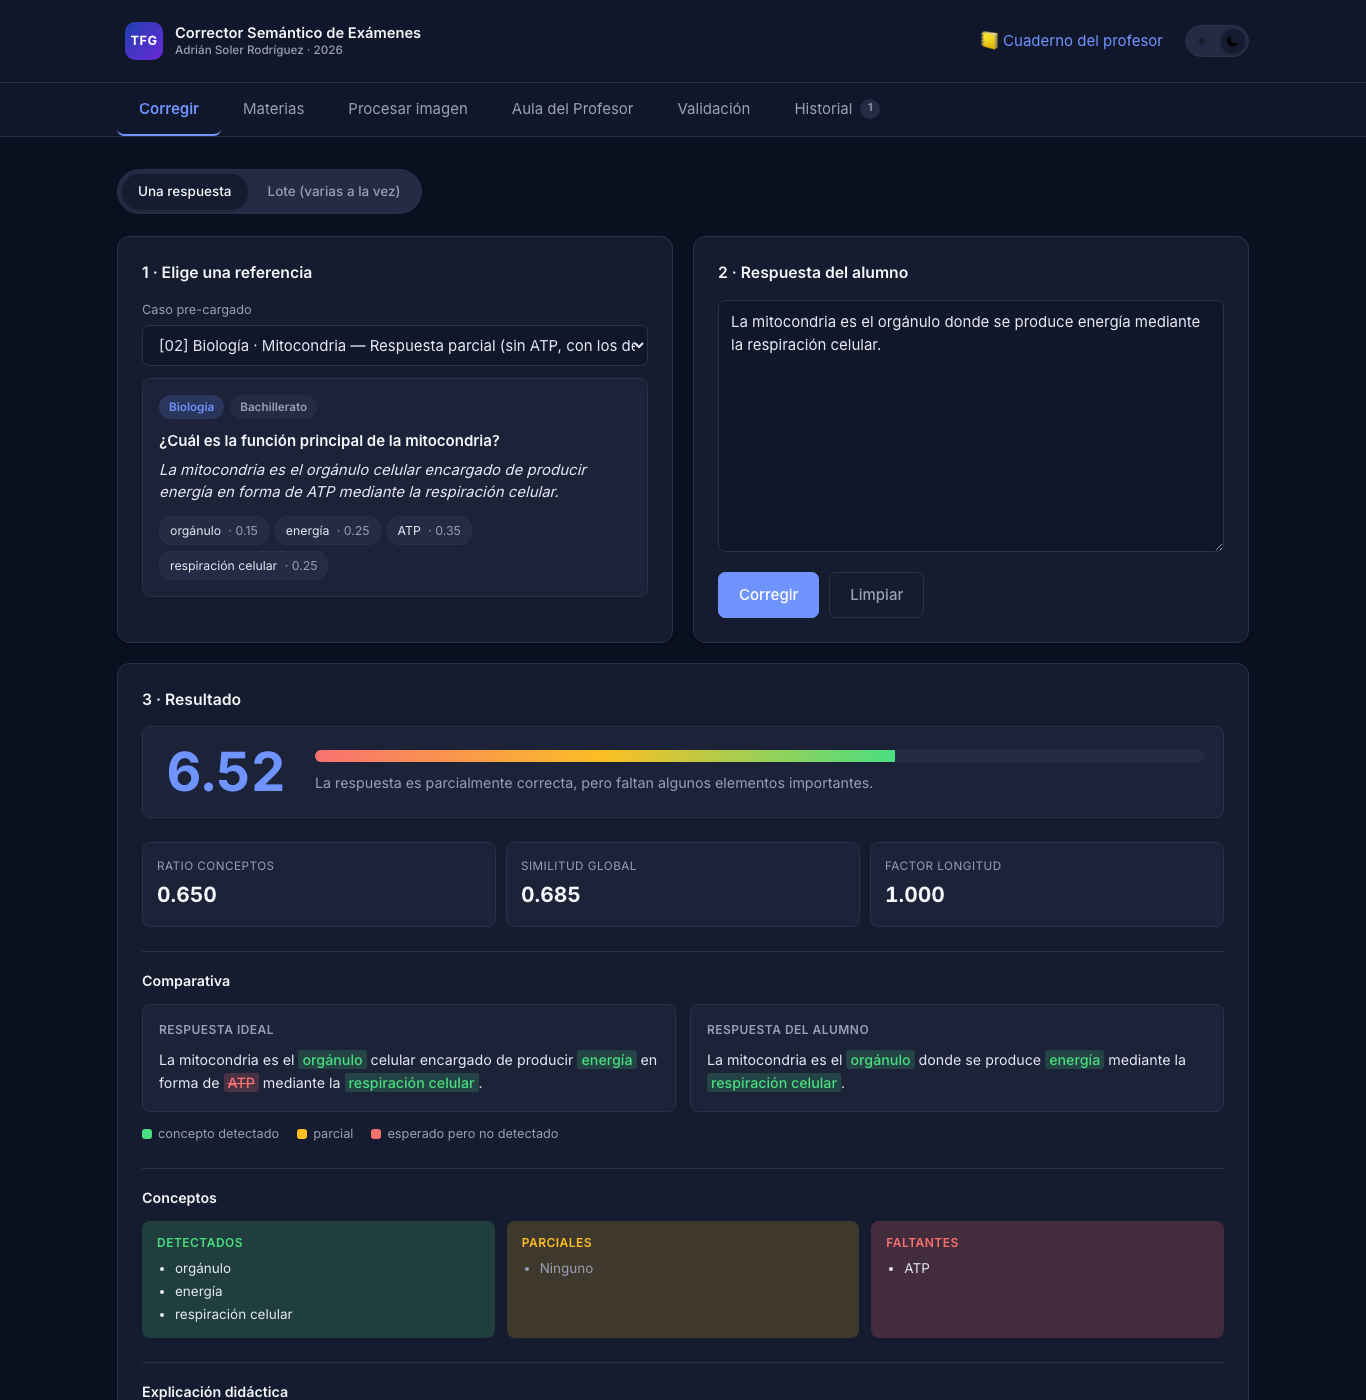
\includegraphics[width=0.92\textwidth]{web_corregir.png}
\caption{Corrección de una respuesta parcial. Se observa la nota (6{,}52), la descomposición en señales y la comparación con la respuesta ideal, con los conceptos detectados, parciales y faltantes diferenciados por color.}
\label{fig:web-corregir}
\end{figure}

La figura~\ref{fig:web-validacion} reproduce la pestaña de validación, que ejecuta la batería de 40 casos y muestra el resumen de conformidad, la distribución por asignatura y por tema, y el detalle de cada caso con su nota y su banda esperada.

\begin{figure}[ht]
\centering
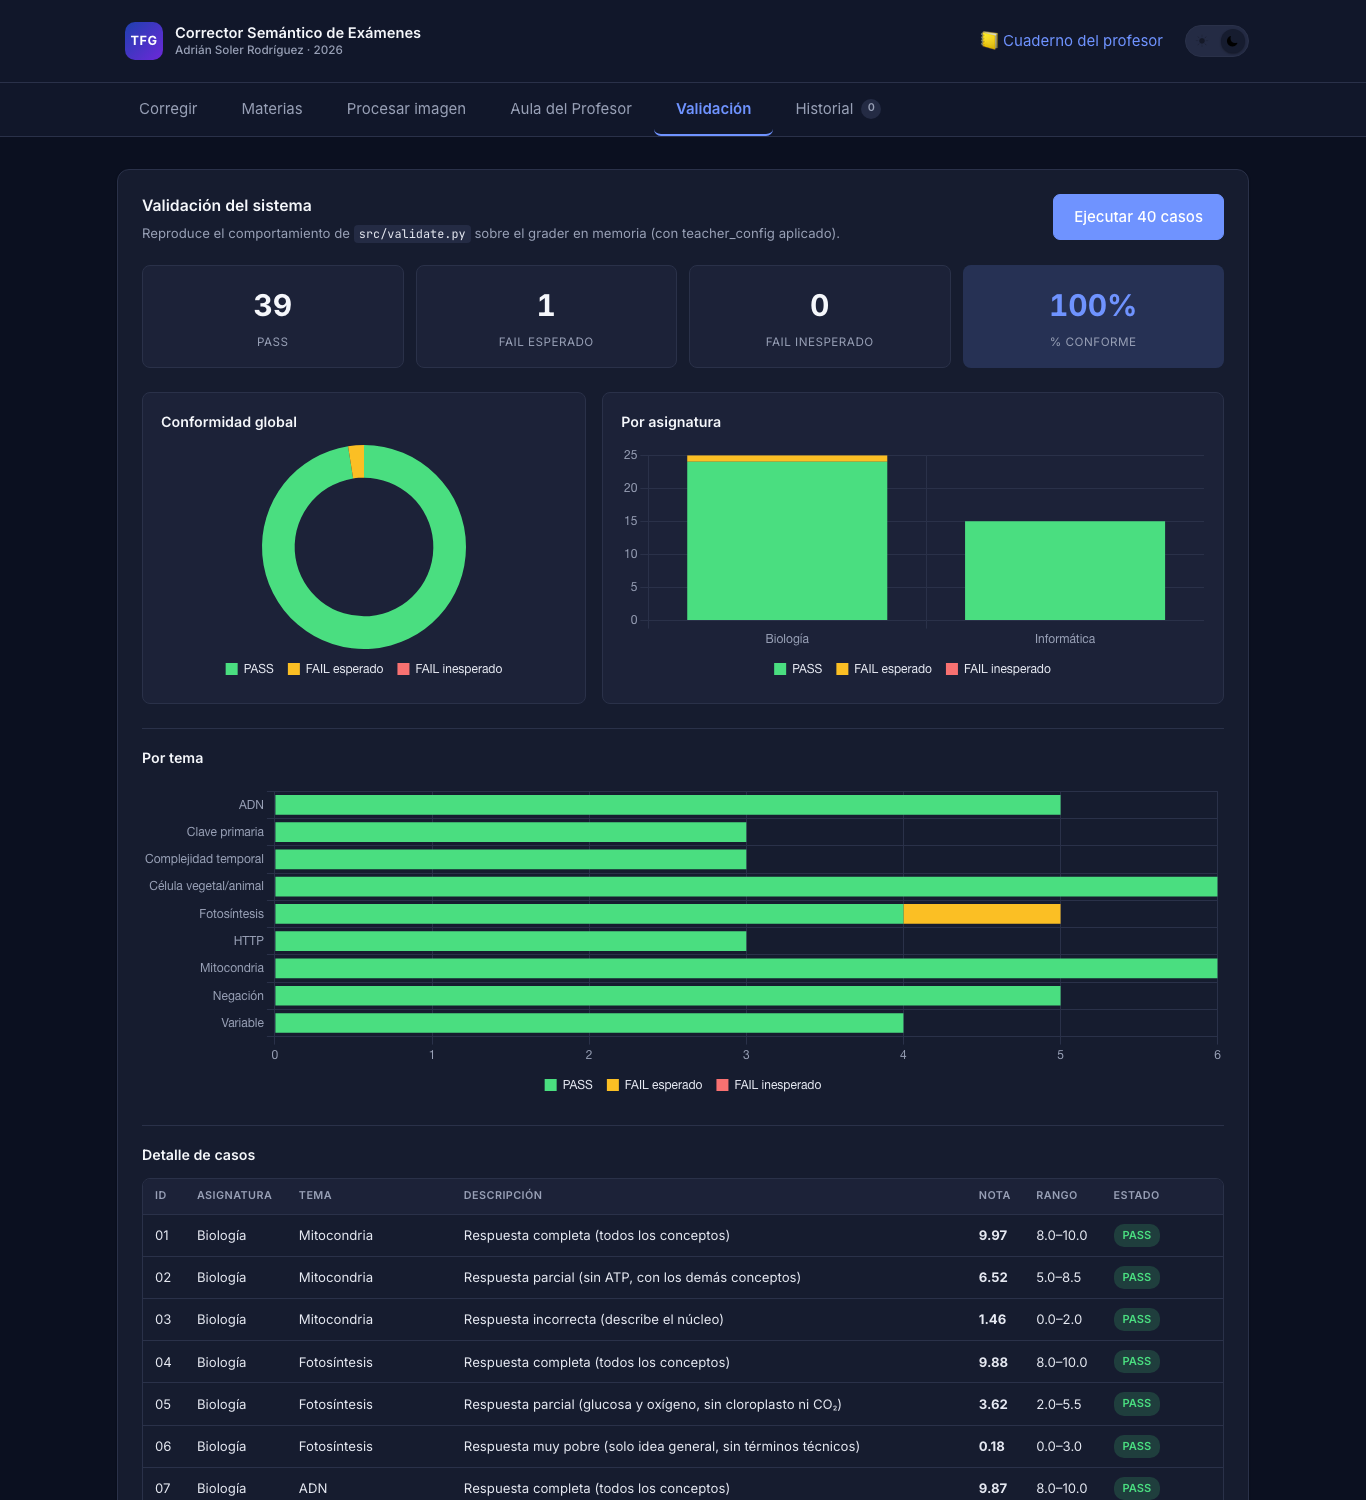
\includegraphics[width=0.92\textwidth]{web_validacion.png}
\caption{Pestaña de validación: resumen de conformidad, gráficos por asignatura y tema, y detalle de casos.}
\label{fig:web-validacion}
\end{figure}

Dentro de la misma pestaña, la herramienta calcula la concordancia con una nota de referencia y la muestra de forma visual. La figura~\ref{fig:web-dispersion} reproduce ese panel: las métricas de correlación y error, un diagrama de dispersión que enfrenta la nota del sistema con la del profesor —con la diagonal de acuerdo perfecto— y el desglose del coeficiente de Spearman por pregunta. Es la versión interactiva de los resultados que se analizan en el capítulo~\ref{cap:resultados}.

\begin{figure}[ht]
\centering
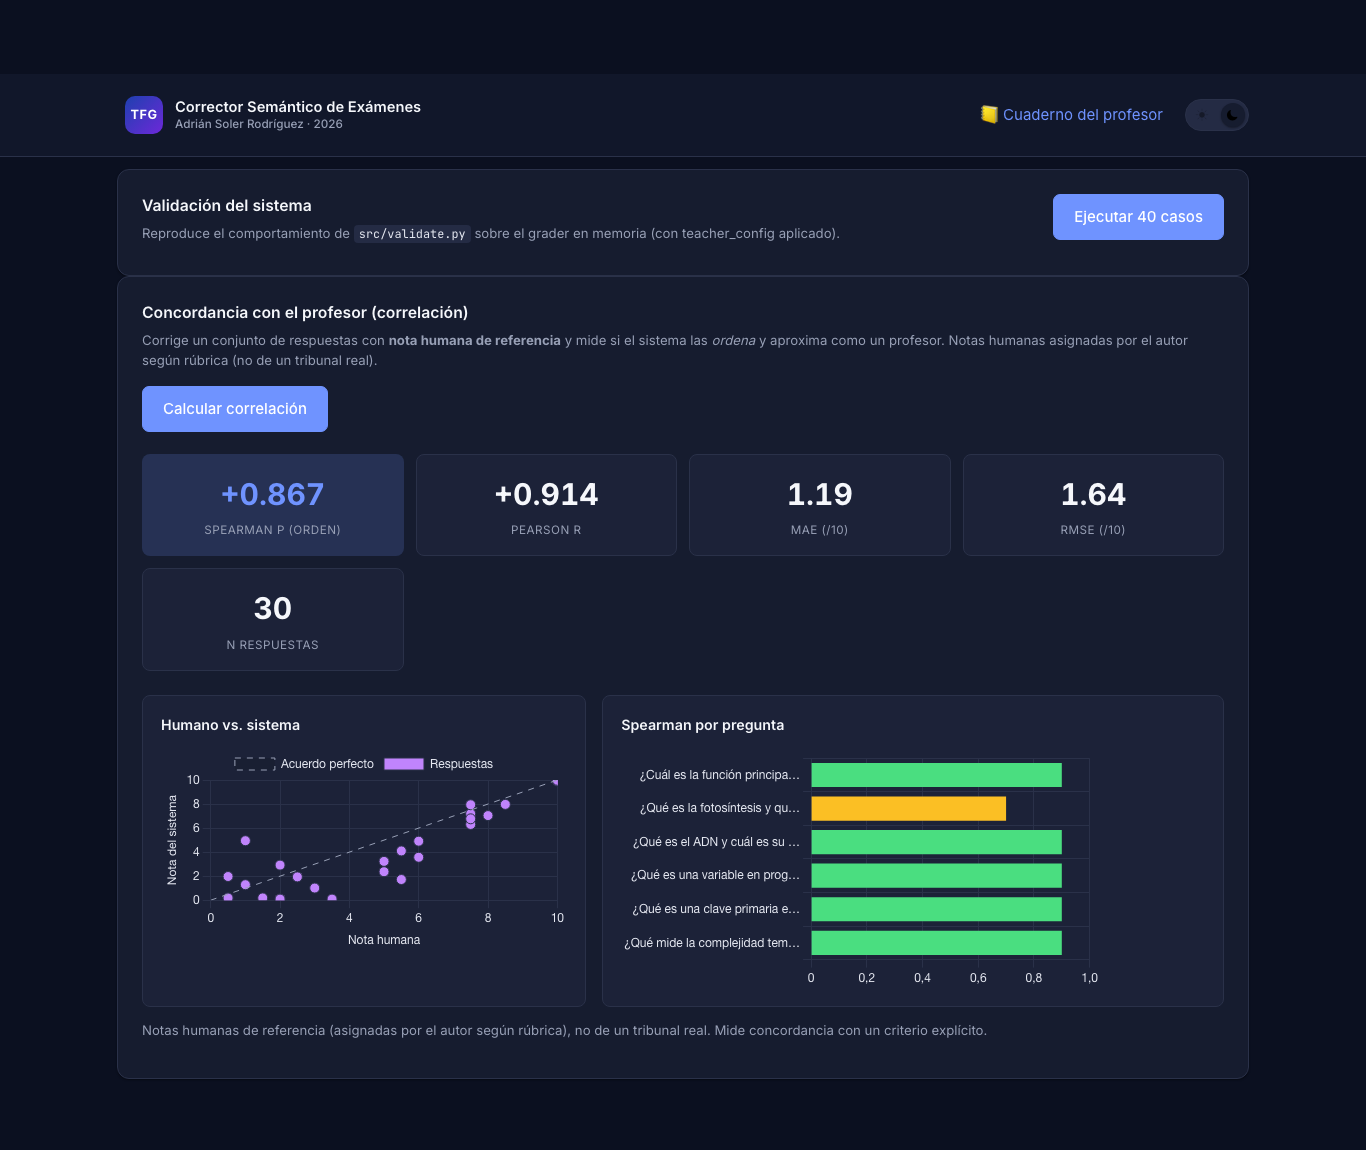
\includegraphics[width=0.92\textwidth]{web_dispersion.png}
\caption{Panel de concordancia: métricas (Spearman, Pearson, MAE, RMSE), diagrama de dispersión nota del sistema frente a nota de referencia con la diagonal de acuerdo perfecto, y Spearman por pregunta.}
\label{fig:web-dispersion}
\end{figure}

\section{Tecnologías y herramientas utilizadas}

El sistema se ha desarrollado en Python por su idoneidad para prototipos que combinan procesamiento de texto, visión por computador e integración de servicios. Las principales tecnologías empleadas son las siguientes:

\begin{itemize}[leftmargin=1.4em]
  \item \textbf{Tesseract} (a través de \texttt{pytesseract}) como motor de reconocimiento óptico de caracteres, y \texttt{OpenCV} y \texttt{Pillow} para las operaciones de imagen.
  \item \textbf{SymPy} para la comparación por equivalencia simbólica en el corrector numérico de Matemáticas y Física.
  \item \textbf{FastAPI} y \texttt{uvicorn} para el \emph{backend} web, con un \emph{frontend} estático en HTML, CSS y JavaScript sin marcos.
  \item Un \textbf{modelo de lenguaje} de la familia Claude, accedido mediante su SDK oficial, para las funciones opcionales de generación de referencia, verificación de factualidad y juez de redacción, siempre con temperatura cero para favorecer la reproducibilidad.
  \item \textbf{pytest} como marco de pruebas, y \texttt{git} para el control de versiones.
\end{itemize}

Una decisión transversal ha sido evitar dependencias pesadas en el núcleo de evaluación. Las métricas de concordancia (Spearman, Pearson, error medio) y la calibración isotónica se han implementado directamente, sin recurrir a bibliotecas de cálculo científico de gran tamaño. Esto mantiene el sistema ligero, facilita su despliegue y es coherente con el principio de interpretabilidad: cada cálculo que interviene en la nota es inspeccionable.

\section{Metodología de desarrollo y validación continua}

El desarrollo siguió un enfoque iterativo guiado por las pruebas. Cada vez que se detectaba un comportamiento incorrecto —una respuesta falsa con nota alta, una paráfrasis infravalorada, un desfase frente a notas humanas— se añadía un caso de prueba que lo capturaba, se modificaba el sistema y se comprobaba que la batería completa seguía pasando. Este ciclo evitó que la corrección de un problema introdujera regresiones en otro, algo especialmente importante en un módulo, el de evaluación, donde un cambio en una heurística puede tener efectos sutiles en muchos casos a la vez.

El proyecto cuenta con una batería de pruebas automáticas que supera las doscientas comprobaciones, entre pruebas unitarias de cada componente —detección de polaridad, sinónimos, métricas, calibración, corrector numérico— y pruebas de integración de los \emph{endpoints} de la API. A ello se suma la batería de validación de 40 casos, que actúa como prueba de aceptación del corrector. Esta red de seguridad fue la que permitió, por ejemplo, detectar de inmediato que el análisis de polaridad introducía un falso positivo en una respuesta de bases de datos, antes de que ese efecto se propagara.

\section{Decisiones de diseño y justificación técnica}

Conviene cerrar el capítulo subrayando que muchas de estas decisiones no surgieron de una planificación previa, sino de problemas observados durante el desarrollo. El preprocesamiento de imagen se moderó tras comprobar que un umbral agresivo deformaba caracteres y hacía desaparecer términos clave. El peso de la similitud global se redujo al ver que los errores de OCR penalizaban respuestas válidas. Se introdujo el suelo mínimo al detectar respuestas correctas que quedaban cerca del suspenso por una baja similitud textual. Se pasó de una lista plana de palabras a conceptos ponderados al comprobar que no todos los términos aportan el mismo valor. Y se añadieron la polaridad, los sinónimos, el verificador y la calibración en respuesta directa a fallos concretos: respuestas que negaban lo correcto, paráfrasis infravaloradas, atribuciones erróneas y desfases de escala frente a un corrector humano. El diseño final responde, por tanto, a limitaciones reales y no a una formulación abstracta previa.

\chapter{Resultados y validación experimental}
\label{cap:resultados}

\section{Diseño de la evaluación}

Para valorar el comportamiento del sistema no basta con indicar que genera una nota. Lo relevante es comprobar cómo responde ante casos representativos, si distingue respuestas correctas, parciales e incorrectas, y hasta qué punto su calificación se aproxima a la de un corrector humano. Por ese motivo la validación se ha planteado en varios niveles, de menor a mayor exigencia: un análisis cualitativo de casos, una batería determinista con notas esperadas, pruebas de robustez ante respuestas tramposas, un banco de exámenes que cubre varios niveles educativos, una medida de concordancia mediante correlación de Spearman frente a notas de referencia y, finalmente, una validación contra notas de profesores humanos reales sobre un conjunto de datos externo.

Conviene una advertencia metodológica que se mantiene a lo largo del capítulo. En las pruebas propias, las notas humanas con las que se compara el sistema son \emph{de referencia}: las ha asignado el autor según rúbrica, emulando el criterio de un profesor del nivel correspondiente. No proceden de un tribunal real. Sirven para medir la concordancia con un criterio explícito, no la exactitud absoluta. La única excepción es la validación externa, donde las notas sí son de correctores humanos reales.

\section{Análisis cualitativo de tres casos}

Como punto de partida se analizan tres respuestas de comportamiento claramente distinto sobre la misma pregunta de biología celular, con los conceptos clave \emph{mitocondria}, \emph{energía}, \emph{ATP} y \emph{respiración celular}. La tabla~\ref{tab:casos} las resume. La primera cubre por completo el contenido; la segunda expresa una comprensión parcial; la tercera utiliza un término del dominio, pero lo relaciona de forma incorrecta.

\begin{table}[ht]
\centering
\caption{Evaluación semántica sobre tres respuestas representativas.}
\label{tab:casos}
\small
\begin{tabularx}{\textwidth}{>{\raggedright\arraybackslash}p{0.16\textwidth} >{\raggedright\arraybackslash}X >{\raggedright\arraybackslash}p{0.10\textwidth}}
\toprule
Tipo & Texto y conceptos & Nota \\
\midrule
Correcta & ``La mitocondria es un orgánulo que produce energía en forma de ATP mediante la respiración celular.'' Detecta todos los conceptos. & 8--10 \\
Parcial & ``La mitocondria produce energía para la célula.'' Detecta mitocondria y energía; respiración celular parcial; ATP ausente. & $\sim 6$ \\
Incorrecta & ``La mitocondria es el núcleo de la célula.'' El término aparece, pero no sostiene una relación válida. & $<4$ \\
\bottomrule
\end{tabularx}
\end{table}

El interés de estos casos es que la diferencia entre ellos no depende de una sola señal, sino de la interacción entre varias decisiones de diseño. La respuesta correcta se beneficia de una cobertura conceptual completa y una similitud alta. La parcial conserva una nota media porque aporta parte del contenido nuclear, pero no encuentra ATP y solo recibe evidencia parcial de \emph{respiración celular}. La incorrecta queda por debajo de 4 porque la mera presencia del término ``mitocondria'' no activa evidencia válida cuando la relación semántica es errónea. Este comportamiento evita uno de los fallos clásicos de la corrección automática: premiar respuestas incorrectas que reutilizan el vocabulario del tema.

\section{Batería de validación determinista}

Para poder detectar regresiones de forma sistemática, se construyó una batería de validación (\texttt{validate.py}) con 40 casos repartidos en dos asignaturas, Biología e Informática, agrupados por tema. Cada caso fija una respuesta y una banda de nota esperada, y se considera conforme si la nota del sistema cae dentro de la banda. La batería incluye respuestas completas, parciales, triviales y adversarias, además de cinco casos específicos de negación y polaridad.

En su estado actual, la batería arroja un comportamiento conforme del 100\,\%: 39 casos pasan dentro de su banda y un único caso falla de forma esperada (está marcado como tal, pues comprueba precisamente una limitación conocida). Esta batería actúa como red de seguridad: cualquier cambio en el grader se contrasta contra ella antes de darse por bueno, lo que permitió, por ejemplo, detectar de inmediato un falso positivo introducido por el análisis de polaridad, descrito más adelante. El conjunto de pruebas del proyecto, ejecutado de forma automática, supera las doscientas comprobaciones unitarias y de integración.

\section{Evaluación del reconocimiento óptico}

Como el sistema parte de imágenes, conviene cuantificar el eslabón del OCR en lugar de darlo por bueno. Para ello se renderizaron respuestas reales del banco con una tipografía estándar y se sometieron a degradaciones típicas de un escaneo o una fotografía —desenfoque, ruido, rotación y baja resolución—, midiendo el error de lectura por carácter (CER) y por palabra (WER), y, sobre todo, la diferencia de nota entre corregir el texto original y corregir el texto leído por OCR. Es importante delimitar el alcance: esta prueba evalúa texto \textbf{impreso}, no manuscrito; el reconocimiento de escritura a mano es un problema distinto y más difícil, reconocido como límite del trabajo. Por tanto, estas cifras son un límite optimista respecto a un examen manuscrito real.

\begin{table}[ht]
\centering
\caption{Robustez del OCR de texto impreso ante degradaciones de imagen (14 respuestas, idioma español).}
\label{tab:ocr}
\small
\begin{tabular}{lccc}
\toprule
Condición & CER & WER & $|\Delta\text{nota}|$ media \\
\midrule
Limpio & 0\,\% & 0\,\% & 0{,}00 \\
Baja resolución & 0{,}8\,\% & 4{,}3\,\% & 0{,}00 \\
Rotación (4\textdegree) & 25{,}2\,\% & 31{,}5\,\% & 0{,}28 \\
Desenfoque & 6{,}8\,\% & 22{,}7\,\% & 1{,}58 \\
Ruido fuerte & 100\,\% & 100\,\% & 9{,}62 \\
\bottomrule
\end{tabular}
\end{table}

La tabla~\ref{tab:ocr} muestra un comportamiento revelador. Con imagen limpia o de baja resolución, el OCR de texto impreso es prácticamente perfecto y la nota no cambia. Lo más interesante es la rotación: produce un 25\,\% de error de caracteres pero solo $0{,}28$ puntos de diferencia en la nota, porque lo que importa para la corrección es que sobrevivan los conceptos clave, no cada letra; el pipeline absorbe el error gracias a la detección parcial y la tolerancia. El ruido fuerte, en cambio, es el punto de ruptura: destruye la lectura y, con ella, la nota. La conclusión es que, para texto impreso en condiciones razonables, el OCR no es el cuello de botella del sistema, y que el módulo semántico aporta una robustez adicional frente a errores moderados de lectura.

\section{Robustez ante respuestas tramposas}

Un corrector serio debe resistir dos trampas que un comparador de conceptos ingenuo no detecta: negar los términos correctos y atribuirlos a otro objeto. La tabla~\ref{tab:robustez} muestra el comportamiento del sistema sobre la pregunta de la mitocondria.

\begin{table}[ht]
\centering
\caption{Comportamiento ante respuestas adversarias (nota sobre 10).}
\label{tab:robustez}
\small
\begin{tabularx}{\textwidth}{>{\raggedright\arraybackslash}X c c}
\toprule
Respuesta del alumno & Sin polaridad & Con el sistema actual \\
\midrule
``La mitocondria \emph{no} produce ATP ni realiza la respiración celular.'' & 9{,}84 & \textbf{0{,}3} \\
``Esos procesos son cosa del cloroplasto, \emph{no} de la mitocondria.'' & 9{,}84 & 9{,}9 + \emph{revisar} \\
``La mitocondria no \emph{solo} produce ATP, sino que respira\dots'' & --- & 9{,}85 \\
\bottomrule
\end{tabularx}
\end{table}

La negación explícita la resuelve el módulo determinista de polaridad: la respuesta falsa cae de 9{,}84 a 0{,}3, mientras que la construcción enfática ``no solo\dots\ sino'' no se penaliza. La atribución errónea, en cambio, escapa a lo determinista —los términos se afirman, solo que referidos al objeto equivocado—; ahí interviene el verificador, que mantiene la nota del grader pero marca el caso para revisión, clasificando los tres conceptos como atribución errónea. La combinación de ambos mecanismos cubre las dos trampas sin volverse indulgente ni injusto con las respuestas correctas que usan negaciones legítimas.

\section{El efecto de los sinónimos: banco de exámenes por nivel}

La prueba más amplia es un banco de exámenes conceptuales (\texttt{exam\_bank.py}) que cubre cinco niveles educativos: Primaria, ESO, Bachillerato, Universidad (Ingeniería Informática) y Máster. Reúne 33 preguntas de un abanico de asignaturas y, para cada una, tres respuestas de alumno —de nivel notable, aprobado y suspenso— con su nota de referencia, lo que suma 99 respuestas calificadas. El sistema corrige cada respuesta y se compara su nota con la de referencia mediante la correlación de Spearman, que mide la concordancia de \emph{orden}, y el error absoluto medio (MAE), que mide la distancia en la escala de 0 a 10.

Este banco fue, además, la prueba que reveló con más claridad la limitación de las paráfrasis descrita en la sección~\ref{sec:sinonimos}: el sistema infravaloraba respuestas correctas expresadas con palabras propias. La tabla~\ref{tab:banco} compara la concordancia antes y después de incorporar los sinónimos por concepto.

\begin{table}[ht]
\centering
\caption{Concordancia con la nota de referencia en el banco por niveles, antes y después de los sinónimos por concepto.}
\label{tab:banco}
\small
\begin{tabular}{lcccc}
\toprule
 & \multicolumn{2}{c}{Sin sinónimos} & \multicolumn{2}{c}{Con sinónimos} \\
\cmidrule(lr){2-3}\cmidrule(lr){4-5}
Métrica (global, $N=99$) & Spearman & MAE & Spearman & MAE \\
\midrule
Resultado & $+0{,}872$ & $1{,}44$ & $\mathbf{+0{,}931}$ & $\mathbf{0{,}96}$ \\
\bottomrule
\end{tabular}
\end{table}

La incorporación de los sinónimos elevó la correlación global de Spearman de $0{,}872$ a $0{,}931$, redujo el error medio de $1{,}44$ a $0{,}96$ puntos sobre 10 y rebajó la proporción de discrepancias importantes (desviaciones de 2{,}5 puntos o más respecto a la referencia) del 24\,\% al 9\,\%. La tabla~\ref{tab:niveles} muestra el detalle por nivel con la versión final del sistema.

\begin{table}[ht]
\centering
\caption{Concordancia por nivel educativo (versión con sinónimos).}
\label{tab:niveles}
\small
\begin{tabular}{lccc}
\toprule
Nivel & $N$ & Spearman & MAE \\
\midrule
Primaria & 15 & $+0{,}95$ & $0{,}72$ \\
ESO & 21 & $+0{,}91$ & $0{,}89$ \\
Bachillerato & 21 & $+0{,}94$ & $1{,}19$ \\
Universidad & 24 & $+0{,}94$ & $1{,}07$ \\
Máster & 18 & $+0{,}92$ & $0{,}81$ \\
\bottomrule
\end{tabular}
\end{table}

\begin{figure}[ht]
\centering
\begin{tikzpicture}
\begin{axis}[
  ybar, bar width=16pt, width=0.85\textwidth, height=5.5cm,
  ymin=0, ymax=1, ylabel={Spearman $\rho$},
  symbolic x coords={Primaria,ESO,Bachillerato,Universidad,Máster},
  xtick=data, x tick label style={font=\footnotesize},
  nodes near coords, nodes near coords style={font=\scriptsize},
  enlarge x limits=0.12]
\addplot[fill=blue!40] coordinates {(Primaria,0.95)(ESO,0.91)(Bachillerato,0.94)(Universidad,0.94)(Máster,0.92)};
\end{axis}
\end{tikzpicture}
\caption{Correlación de Spearman por nivel educativo (versión con sinónimos).}
\label{fig:spearman-nivel}
\end{figure}

El sistema ordena las respuestas como un corrector de referencia en todos los niveles, de Primaria a Máster, sin que la correlación caiga en ningún tramo por debajo de $0{,}91$ (figura~\ref{fig:spearman-nivel}). El banco fue también útil para depurar el sistema: destapó un falso positivo del detector de negación, en el que el ``no'' de ``no metales'' marcaba como negados los conceptos posteriores de una respuesta de Química y hundía un notable de 10 a 6; el error se corrigió añadiendo ``no metales'' a las excepciones léxicas. De las nueve discrepancias que quedan, dos son sobrevaloraciones por presencia de términos sin coherencia —las que marca el verificador— y siete son infravaloraciones de respuestas genuinamente incompletas, donde el alumno solo nombra parte de la rúbrica; que una respuesta a medias obtenga menos nota que una completa es el comportamiento correcto. La tabla~\ref{tab:discrep} las clasifica.

\begin{table}[ht]
\centering
\caption{Clasificación de las nueve discrepancias restantes en el banco por niveles.}
\label{tab:discrep}
\small
\begin{tabularx}{\textwidth}{>{\raggedright\arraybackslash}p{0.28\textwidth} c >{\raggedright\arraybackslash}X}
\toprule
Asignatura / nivel & Tipo & Causa \\
\midrule
Lengua (ESO) & Sobrevalora & Términos correctos en una afirmación falsa \\
Biología (Bach.) & Sobrevalora & ``Consume oxígeno'': proceso invertido \\
Estructuras de Datos (Univ.) & Infravalora & Respuesta incompleta (solo el concepto central) \\
Sistemas Operativos (Univ.) & Infravalora & Respuesta incompleta \\
Filosofía (Bach.) $\times 2$ & Infravalora & No reproduce el término técnico exacto \\
Programación (Univ.) & Infravalora & Respuesta incompleta \\
Machine Learning (Máster) & Infravalora & Respuesta incompleta \\
Matemáticas (Bach.) & Infravalora & Falta un concepto de la rúbrica \\
\bottomrule
\end{tabularx}
\end{table}

Las dos sobrevaloraciones son, precisamente, los casos para los que existe el verificador; las infravaloraciones reflejan respuestas a las que un profesor concede el beneficio de la duda y que el sistema, más literal, califica algo por debajo. Ninguna de las dos categorías es un fallo de funcionamiento: delimitan el margen de error esperable.

\section{Correlación de Spearman sobre un conjunto de referencia}

Para disponer de una medida de concordancia más exigente que las bandas de la batería determinista, se construyó un conjunto de 30 respuestas con nota de referencia repartida por toda la escala, sobre seis preguntas de Biología e Informática (\texttt{gold\_dataset.py}). Sobre este conjunto, el sistema obtiene una correlación de Spearman de $0{,}87$, una correlación de Pearson de $0{,}91$ y un error medio de $1{,}2$ puntos sobre 10. El propio experimento expone, además, las costuras del enfoque: una pregunta de fotosíntesis baja su correlación porque una respuesta incorrecta que ``consume oxígeno'' es sobrevalorada por presencia de términos, un caso que el verificador detectaría. La figura~\ref{fig:scatter} representa la nota del sistema frente a la de referencia para las 30 respuestas; la diagonal marca el acuerdo perfecto. La mayoría de los puntos se sitúan cerca de ella, y las desviaciones se concentran en la zona media, coherentes con la tendencia del sistema a ser algo más severo con las respuestas intermedias.

\begin{figure}[ht]
\centering
\begin{tikzpicture}
\begin{axis}[
  width=0.8\textwidth, height=7cm,
  xlabel={Nota de referencia (humano)}, ylabel={Nota del sistema},
  xmin=0,xmax=10,ymin=0,ymax=10, grid=both, grid style={gray!20},
  legend pos=north west, legend style={font=\footnotesize}]
\addplot[domain=0:10, dashed, gray, thick, forget plot] {x};
\addplot[only marks, mark=*, mark size=1.6pt, blue!70] coordinates {
 (10,9.99)(7.5,6.3)(5.5,4.1)(2.5,1.94)(0.5,1.97)
 (10,9.97)(8.5,7.97)(6,4.91)(3,1.01)(1,4.95)
 (10,9.96)(7.5,7.19)(5,3.23)(2,0.11)(0.5,0.19)
 (10,9.97)(7.5,7.94)(5,2.37)(2,0.09)(0.5,0.18)
 (10,9.91)(7.5,6.77)(5.5,1.72)(1.5,0.19)(2,2.92)
 (10,9.98)(8,7.04)(6,3.57)(3.5,0.09)(1,1.29)};
\legend{Respuestas}
\end{axis}
\end{tikzpicture}
\caption{Nota del sistema frente a la nota de referencia sobre el conjunto de 30 respuestas. La diagonal discontinua indica el acuerdo perfecto.}
\label{fig:scatter}
\end{figure}

Estas métricas se calculan con una implementación propia de los coeficientes (\texttt{metrics.py}), sin dependencias pesadas, lo que mantiene la coherencia con el carácter interpretable del resto del sistema.

\section{Validación con datos reales: el conjunto de Mohler}

Hasta este punto, todas las notas humanas eran de referencia. La prueba definitiva es contrastar el sistema con notas de profesores humanos reales. Para ello se utilizó el conjunto de \textcite{mohler2011}: 87 preguntas de un curso universitario de informática, en inglés, con unas 2.400 respuestas de alumnos calificadas por dos correctores humanos. El sistema corrige cada respuesta —derivando los conceptos de forma automática a partir de la respuesta de referencia— y se mide su concordancia con la nota humana.

Es importante interpretar este resultado como un \emph{suelo}, no como el mejor caso. El conjunto está en inglés, donde las funciones de negación y sinónimos, diseñadas para el español, no actúan, de modo que solo se prueba el motor base. Además, la rúbrica se deriva automáticamente y es más pobre que una construida por un profesor. La tabla~\ref{tab:mohler} recoge los resultados.

\begin{table}[ht]
\centering
\caption{Concordancia con notas humanas reales (conjunto de Mohler, $N \approx 2400$).}
\label{tab:mohler}
\small
\begin{tabular}{lc}
\toprule
Métrica & Valor \\
\midrule
Spearman global & $+0{,}54$ \\
Pearson & $+0{,}48$ \\
MAE & $4{,}33$ / 10 \\
MAE tras corregir el sesgo de escala & $\mathbf{1{,}63}$ / 10 \\
\bottomrule
\end{tabular}
\end{table}

El dato más informativo no es el error bruto, sino su naturaleza. La media de las notas humanas es $8{,}38$ y la del sistema $4{,}15$: un desfase de más de cuatro puntos. Los correctores de Mohler son muy generosos —el 80\,\% de sus notas son iguales o superiores a 7—, mientras que el sistema es estricto. Al restar ese desfase constante, el error medio cae de $4{,}33$ a $1{,}63$. En otras palabras, el sistema \emph{ordena} las respuestas de forma parecida a los humanos, pero en una escala más severa. El error es sobre todo de escala, no de criterio.

\section{El techo humano: el acuerdo entre dos correctores}

La cifra anterior puede leerse como decepcionante solo si se compara con un ideal de correlación 1. Pero ese ideal no existe ni siquiera entre humanos. El conjunto de Mohler proporciona, además del promedio, las notas de \emph{los dos correctores por separado}, lo que permite la comparación más directa posible: medir cuánto concuerdan los dos profesores entre sí. Esa concordancia humano-humano es el \emph{techo} realista al que puede aspirar cualquier sistema.

Sobre las respuestas con alineamiento verificado entre respuesta y notas (1.868 respuestas), los dos correctores humanos concuerdan con una correlación de Spearman de \textbf{0,60}. El sistema alcanza \textbf{0,55} con el promedio humano. La tabla~\ref{tab:techo} lo resume, con intervalos de confianza al 95\,\% obtenidos por \emph{bootstrap}.

\begin{table}[ht]
\centering
\caption{Concordancia humano-humano (techo) frente a la del sistema, conjunto de Mohler.}
\label{tab:techo}
\small
\begin{tabularx}{\textwidth}{>{\raggedright\arraybackslash}X c c}
\toprule
Comparación & Spearman (IC 95\,\%) & MAE \\
\midrule
Humano 1 vs. Humano 2 (\textbf{techo}) & $+0{,}60$ $[0{,}57,\,0{,}64]$ & $1{,}42$ \\
Sistema vs. promedio humano & $+0{,}55$ $[0{,}52,\,0{,}58]$ & $4{,}39$ \\
Sistema vs. Humano 1 & $+0{,}50$ $[0{,}47,\,0{,}54]$ & $4{,}16$ \\
Sistema vs. Humano 2 & $+0{,}49$ $[0{,}45,\,0{,}52]$ & $4{,}81$ \\
\bottomrule
\end{tabularx}
\end{table}

La figura~\ref{fig:techo} representa estas cifras con sus intervalos de confianza, junto a la línea que marca el techo humano. Se aprecia visualmente que las barras del sistema no quedan lejos de ese techo.

\begin{figure}[ht]
\centering
\begin{tikzpicture}
\begin{axis}[
  ybar, bar width=26pt, width=0.85\textwidth, height=6.2cm,
  ymin=0, ymax=0.75, ylabel={Spearman $\rho$},
  symbolic x coords={H1 vs H2, Sist vs prom, Sist vs H1, Sist vs H2},
  xtick=data, x tick label style={font=\footnotesize},
  enlarge x limits=0.18, legend pos=north east, legend style={font=\footnotesize}]
\addplot+[fill=blue!40, draw=blue!60,
         nodes near coords, nodes near coords style={font=\scriptsize},
         error bars/.cd, y dir=both, y explicit]
  coordinates {
    (H1 vs H2,0.60) +- (0,0.035)
    (Sist vs prom,0.55) +- (0,0.03)
    (Sist vs H1,0.50) +- (0,0.035)
    (Sist vs H2,0.49) +- (0,0.035)};
\addplot[dashed, red!70, thick, mark=none] coordinates {(H1 vs H2,0.60) (Sist vs H2,0.60)};
\legend{$\rho$ (IC 95\,\%), Techo humano}
\end{axis}
\end{tikzpicture}
\caption{Acuerdo humano-humano (techo) frente al del sistema sobre el conjunto de Mohler, con intervalos de confianza al 95\,\%. La línea discontinua marca el techo humano ($\rho=0{,}60$).}
\label{fig:techo}
\end{figure}

La lectura cambia por completo. El sistema no concuerda con el promedio humano un poco peor que un humano: concuerda a $0{,}55$ cuando el techo humano es $0{,}60$, es decir, alcanza en torno al \textbf{90\,\% del acuerdo que dos profesores tienen entre sí}, y lo hace en su peor escenario (inglés, rúbrica derivada automáticamente, sin sinónimos). Visto contra ese techo, el resultado deja de ser una cifra pobre y pasa a ser notable. Este es, probablemente, el resultado más importante del trabajo, porque sustituye una comparación con un ideal imposible por una comparación con la realidad: la corrección humana tampoco es perfectamente consistente.

\section{Recalibración sobre datos reales}

El hallazgo anterior justifica la capa de calibración de la sección~\ref{sec:calibracion}. Para comprobar que el desfase se corrige sin circularidad —entrenando y midiendo en datos distintos—, se entrenó el calibrador con el 70\,\% del conjunto de Mohler y se evaluó sobre el 30\,\% restante, no visto durante el ajuste. La tabla~\ref{tab:calibracion} muestra el resultado en ese conjunto de prueba.

\begin{table}[ht]
\centering
\caption{Efecto de la calibración sobre el 30\,\% de Mohler no usado en el ajuste.}
\label{tab:calibracion}
\small
\begin{tabular}{lccc}
\toprule
 & MAE & Pearson & Spearman \\
\midrule
Sin calibrar & $4{,}18$ & $+0{,}47$ & $+0{,}53$ \\
Calibración lineal & $\mathbf{1{,}42}$ & $+0{,}48$ & $+0{,}53$ \\
Calibración isotónica & $1{,}46$ & $+0{,}45$ & $+0{,}53$ \\
\bottomrule
\end{tabular}
\end{table}

El error medio sobre datos no vistos cae de $4{,}18$ a $1{,}42$, lo que demuestra que el desfase era sistemático y se corrige con muy pocas notas del profesor. La correlación de Spearman no cambia, como era de esperar de un mapeo monótono: la calibración no inventa orden, solo ajusta la escala. Ahora bien, conviene no perder de vista un matiz importante. El calibrador lineal ajustado fue, aproximadamente, $\mathrm{nota} = 0{,}34 \cdot \mathrm{cruda} + 7{,}0$, lo que lleva una respuesta cruda de 0 a un 7. Esto no es un defecto del método, sino su consecuencia lógica: la calibración reproduce la generosidad de los correctores de Mohler, incluida su escasa discriminación. La lección es clara: la calibración corrige el desajuste de escala, pero es tan exigente como las notas que la alimentan, y por eso conviene combinarla con rúbricas y sinónimos curados, que sí discriminan.

\section{Enrutado por tipo de pregunta}

Las pruebas anteriores se centran en preguntas conceptuales, que son el ámbito del corrector semántico. Para comprobar el comportamiento sobre un examen heterogéneo se preparó una prueba con preguntas de estilo EvAU de ocho asignaturas, mezclando definiciones, cálculo numérico y redacción. Al pasar \emph{todas} por el corrector semántico, el sistema funcionaba bien en las asignaturas conceptuales (Historia, Filosofía, Química, Economía, Biología) pero fallaba de forma sistemática en cálculo (Matemáticas) y en redacción (Lengua, Lengua extranjera), donde premiaba las palabras clave aunque el resultado fuese incorrecto o la expresión deficiente.

Al activar el enrutado por tipo —corrector semántico para lo conceptual, corrector numérico por equivalencia para el cálculo y juez con rúbrica para la redacción—, las respuestas que antes quedaban mal calificadas pasaron a situarse en la banda que asignaría un profesor. La tabla~\ref{tab:router} resume el cambio: el corrector numérico distingue una conclusión errónea ($x=3$) de la correcta ($x=-3$) aunque ambas citen el símbolo, y el juez de redacción hunde un texto gramaticalmente pobre aunque contenga todo el vocabulario esperado.

\begin{table}[ht]
\centering
\caption{Efecto del enrutado por tipo de pregunta sobre un examen heterogéneo.}
\label{tab:router}
\small
\begin{tabularx}{\textwidth}{>{\raggedright\arraybackslash}p{0.22\textwidth} >{\raggedright\arraybackslash}X c c}
\toprule
Asignatura & Corrector adecuado & Solo semántico & Híbrido \\
\midrule
Historia, Filosofía, Química, Economía, Biología & Semántico & Correcto & Correcto \\
Matemáticas (cálculo) & Numérico (SymPy) & Incorrecto & Correcto \\
Lengua, Lengua extranjera & Juez con rúbrica & Incorrecto & Correcto \\
\bottomrule
\end{tabularx}
\end{table}

La lectura es que el corrector determinista no debe aplicarse indiscriminadamente: su valor está en lo conceptual, y reconocer esa frontera —derivando el resto a un componente específico— es parte del diseño del sistema.

\section{Comparación con una línea base de palabras clave}

Para situar el valor de las mejoras incorporadas conviene compararlas con la alternativa más simple: una corrección por presencia de palabras clave, sin polaridad, sin sinónimos y sin similitud global. Esa línea base, equivalente a comprobar si los términos de la rúbrica aparecen en la respuesta, falla precisamente en los casos que distinguen a un buen corrector de uno ingenuo.

Para cuantificarlo se compararon, sobre el mismo banco, tres correctores: el de solo palabras clave, uno de similitud TF-IDF entre la respuesta y la respuesta ideal (una línea base de similitud más fuerte que la bolsa de palabras, pero que ignora la rúbrica) y el sistema completo. La tabla~\ref{tab:baselines} recoge el resultado, con intervalos de confianza por \emph{bootstrap}.

\begin{table}[ht]
\centering
\caption{Líneas base frente al sistema completo sobre el banco por niveles ($N=99$).}
\label{tab:baselines}
\small
\begin{tabular}{lcc}
\toprule
Método & Spearman (IC 95\,\%) & MAE \\
\midrule
Solo palabras clave & $+0{,}86$ $[0{,}78,\,0{,}92]$ & $1{,}64$ \\
TF-IDF coseno & $+0{,}84$ $[0{,}76,\,0{,}89]$ & $2{,}19$ \\
\textbf{Sistema completo} & $\mathbf{+0{,}93}$ $[0{,}89,\,0{,}95]$ & $\mathbf{0{,}96}$ \\
\bottomrule
\end{tabular}
\end{table}

El sistema supera a ambas líneas base, y la diferencia es mayor en el error medio (0,96 frente a 1,64 y 2,19) que en el orden. Conviene matizar: sobre respuestas conceptuales \emph{limpias} como las del banco, la línea base de palabras clave no es mala ($0{,}86$). Su fragilidad aflora en los casos que el banco no recoge y que sí están en la batería de robustez: en la tabla~\ref{tab:robustez} se vio que una línea base de este tipo otorga un 9{,}84 a una respuesta que niega todo el contenido, mientras que el análisis de polaridad la reduce a 0{,}3. La similitud TF-IDF, por su parte, al ignorar la rúbrica no penaliza lo erróneo ni distingue qué concepto importa. La conclusión es que las mejoras no son adornos: corrigen los errores que harían inservible una corrección simple en un examen real, y lo hacen además mejorando la concordancia agregada.

\section{Reproducibilidad de los resultados}

Una preocupación legítima en cualquier sistema que incorpore un modelo de lenguaje es la reproducibilidad: si las cifras cambian de una ejecución a otra, dejan de ser comparables. En este trabajo, las pruebas que sustentan las tablas anteriores son deterministas, porque el núcleo de corrección lo es: la misma respuesta produce siempre la misma nota. Las funciones que sí dependen de un modelo de lenguaje se invocan con temperatura cero para minimizar su variabilidad, y no intervienen en las métricas de concordancia del corrector, que se calculan únicamente con el grader determinista.

Además, todos los experimentos descritos son reproducibles a partir de los datos incluidos en el proyecto: la batería de validación, el banco de exámenes y los conjuntos de referencia están versionados junto al código, y la validación externa descarga su conjunto de datos de una fuente pública. La separación entre datos y lógica, y la implementación propia de las métricas, hacen que cualquier persona pueda volver a obtener las mismas cifras, lo que es coherente con el énfasis del trabajo en la interpretabilidad y la transparencia de los resultados.

\section{Coste y rendimiento}

Un aspecto a menudo ignorado en la evaluación de un corrector es su coste de ejecución. El núcleo determinista de este sistema realiza, por respuesta, operaciones de texto de complejidad muy baja: normalización, búsqueda de conceptos y un cálculo de similitud sobre vectores de frecuencias. En la práctica, esto significa que la corrección de una respuesta es prácticamente instantánea y que la batería completa de 40 casos, o las 99 respuestas del banco por niveles, se procesan en una fracción de segundo en un equipo personal corriente. El conjunto completo de más de doscientas pruebas automáticas se ejecuta en torno a un segundo.

Este coste contrasta con el de una solución que dependiera de un modelo de lenguaje para cada calificación, donde cada respuesta implicaría una llamada de red, una latencia apreciable y un consumo de recursos varios órdenes de magnitud mayor. Reservar el modelo de lenguaje para funciones opcionales —generación de rúbricas, verificación y juez de redacción— mantiene el coste del flujo principal en niveles despreciables, lo que tiene implicaciones prácticas (la herramienta puede usarse sin coste por uso) y de sostenibilidad. En un escenario de corrección masiva, esta diferencia de coste no es un detalle, sino un factor que condiciona la viabilidad del sistema.

\section{Discusión}

La tabla~\ref{tab:resumen} consolida en un único lugar las medidas de concordancia obtenidas en los distintos escenarios de validación, lo que facilita una lectura comparada.

\begin{table}[ht]
\centering
\caption{Resumen de la validación de concordancia en los distintos escenarios.}
\label{tab:resumen}
\small
\begin{tabularx}{\textwidth}{>{\raggedright\arraybackslash}X c c c}
\toprule
Escenario & $N$ & Spearman & MAE \\
\midrule
Conjunto de referencia (gold) & 30 & $+0{,}87$ & $1{,}2$ \\
Banco por niveles (sin sinónimos) & 99 & $+0{,}87$ & $1{,}44$ \\
Banco por niveles (con sinónimos) & 99 & $\mathbf{+0{,}93}$ & $\mathbf{0{,}96}$ \\
Datos reales (Mohler, sin calibrar) & 1868 & $+0{,}55$ & $4{,}39$ \\
Datos reales (Mohler, calibrado, test) & 733 & $+0{,}53$ & $1{,}42$ \\
\textit{Techo humano-humano (Mohler)} & 1868 & \textit{$+0{,}60$} & \textit{$1{,}42$} \\
\bottomrule
\end{tabularx}
\end{table}

La última fila es la referencia que da sentido al resto: el techo humano-humano. Frente a él, el $0{,}55$ del sistema sobre datos reales no es un suspenso, sino aproximadamente el 90\,\% del acuerdo entre dos profesores.

El conjunto de resultados dibuja un sistema con un comportamiento bien delimitado. Sobre preguntas conceptuales con rúbrica curada y sinónimos —su escenario de diseño— concuerda con la nota de referencia con una correlación de Spearman en torno a $0{,}93$ y un error medio inferior a un punto, de forma consistente en cinco niveles educativos. Resiste las dos trampas clásicas de la corrección por palabras clave gracias a la polaridad determinista y al verificador. Y cuando se enfrenta a datos reales en su peor escenario —otro idioma, sin rúbrica curada— mantiene una concordancia de orden moderada y un error que es casi todo de escala, recuperable con la capa de calibración.

Esa caracterización es, en sí misma, un resultado. La diferencia entre el $0{,}93$ del banco propio y el $0{,}54$ de Mohler no es una contradicción, sino una medida de cuánto dependen el rendimiento de la calidad de la rúbrica y de las funciones específicas del idioma. Antes que presumir de una corrección ``perfecta'', el sistema cuantifica con números cuándo es fiable y cuándo necesita la intervención del profesor, ya sea curando la rúbrica, declarando sinónimos o aportando unas pocas notas para calibrar. Para un sistema pensado como apoyo a la docencia, y no como sustituto del criterio humano, ese reconocimiento de los límites es preferible a una cifra alta sin contexto.

\chapter{Consideraciones éticas, legales y de sostenibilidad}
\label{cap:consideraciones}

Un sistema que interviene en la calificación de exámenes afecta a personas, así que conviene revisar sus implicaciones éticas, legales y de sostenibilidad, varias de las cuales han condicionado decisiones de diseño concretas.

\section{Transparencia y papel del docente}

La decisión más relevante en términos éticos es que cada nota pueda explicarse: una calificación que es una caja negra resulta difícil de defender ante una reclamación. Aquí la nota se descompone en los conceptos detectados, los ausentes y los negados, y la capa basada en un modelo de lenguaje se limita a verificar, sin reescribir la calificación. Coherente con ello, la herramienta se concibe como apoyo y no como sustituto: ordena y propone, pero la última palabra es del docente, lo que evita delegar en una máquina una responsabilidad —evaluar a una persona— que debe seguir siendo humana.

\section{Sesgos y limitaciones}

Todo sistema de evaluación automática puede introducir sesgos, y conviene ser explícito sobre ellos. El corrector premia la presencia de una terminología concreta, lo que podría perjudicar a alumnos que expresan ideas correctas con otro vocabulario; los sinónimos por concepto mitigan ese efecto, pero dependen de que el profesor los declare. Además, la dependencia del OCR implica que la calidad de la letra o del escaneo puede influir en la nota, un factor ajeno al conocimiento del alumno. Por eso la salida debe entenderse como una propuesta revisable, especialmente en decisiones con consecuencias académicas importantes.

\section{Protección de datos}

Los exámenes contienen datos personales, por lo que su tratamiento queda sujeto al Reglamento General de Protección de Datos. El diseño favorece el cumplimiento: la corrección funciona de forma local, sin enviar información a servicios externos, y solo las funciones opcionales basadas en un modelo de lenguaje implican comunicación con un tercero, claramente acotadas y prescindibles. En un despliegue real convendría minimizar los datos enviados, anonimizar las respuestas cuando sea posible e informar a los implicados del tratamiento.

\section{Sostenibilidad}

El coste computacional del corrector es muy bajo: una corrección no requiere inferencia sobre un modelo grande, sino operaciones de texto sencillas, con un consumo energético reducido frente a una solución que dependiera de un modelo de lenguaje para cada calificación. Reservar ese modelo para funciones acotadas limita el impacto energético, un criterio cada vez más relevante en el diseño de software.

\chapter{Conclusiones y trabajo futuro}
\label{cap:conclusiones}

\section{Conclusiones}

Este trabajo ha permitido desarrollar un sistema automático de corrección de preguntas abiertas a partir de imágenes de exámenes, abordando el problema como un \emph{pipeline} completo y no como una suma aislada de técnicas. La propuesta integra procesamiento de imagen, OCR, parseo estructural, generación de referencia, evaluación semántica y producción de \emph{feedback}, y se ha enriquecido con varios mecanismos que responden a limitaciones observadas durante las pruebas.

La principal aportación se encuentra en la estrategia de evaluación semántica. En lugar de reducir la corrección a una coincidencia de palabras, se ha planteado un mecanismo mixto que valora conceptos clave ponderados, proximidad global y adecuación de la extensión, y que se ha mantenido deliberadamente determinista e interpretable. Sobre esa base se han añadido cuatro mejoras que, en conjunto, transforman un comparador de conceptos ingenuo en un corrector razonablemente robusto: el análisis de polaridad, que impide acreditar conceptos negados; los sinónimos por concepto, que reconocen paráfrasis sin perder trazabilidad; el verificador de factualidad, que marca atribuciones erróneas como segunda opinión sin reescribir la nota; y la capa de calibración, que ajusta la escala del sistema al criterio de cada corrector.

La validación respalda estas decisiones con números. En su escenario de diseño —preguntas conceptuales con rúbrica curada—, el sistema concuerda con la nota de referencia con una correlación de Spearman cercana a $0{,}93$ y un error medio inferior a un punto sobre diez, de forma estable desde Primaria hasta Máster. Frente a respuestas adversarias, la polaridad y el verificador evitan los dos fallos clásicos de la corrección por palabras clave. Y la prueba con datos reales de Mohler, lejos de maquillarse, se ha utilizado para mostrar abiertamente el peor caso del sistema y para demostrar que su error es fundamentalmente de escala, corregible mediante calibración.

Otra conclusión relevante, ya presente en la primera versión del proyecto y confirmada después, es que la calidad del OCR condiciona de forma determinante el comportamiento global: la capacidad del módulo semántico no compensa por completo una extracción textual deficiente, por lo que la robustez debe entenderse como una propiedad del \emph{pipeline} entero. En la misma línea, el trabajo ha mostrado que ciertas intuiciones habituales —como que un preprocesamiento de imagen más agresivo siempre mejora la lectura— no se sostienen al contrastarlas empíricamente.

En conjunto, el sistema no sustituye el criterio docente, pero sí ofrece una herramienta con potencial para reducir carga de trabajo, homogeneizar criterios básicos y servir de apoyo en la evaluación, siempre que se reconozcan sus límites. En definitiva, un corrector automático útil no es el que afirma ser perfecto, sino el que explica por qué califica como califica y dónde necesita ayuda.

\section{Lecciones aprendidas}

Más allá del resultado técnico, el desarrollo dejó algunas lecciones que conviene recoger. La primera es que las intuiciones deben contrastarse: la creencia de que un preprocesamiento de imagen más agresivo mejora siempre el OCR resultó falsa en este caso, y solo las pruebas lo revelaron. La segunda es el valor de una batería de pruebas como red de seguridad; en un módulo donde un cambio en una heurística puede alterar muchos casos a la vez, poder comprobar de inmediato que no se ha roto nada fue lo que permitió iterar con confianza. La tercera, quizá la más importante, es que un sistema de evaluación gana más siendo honesto sobre sus límites que aparentando una precisión que no tiene: convertir la prueba con datos reales —donde el sistema rendía peor— en un análisis del porqué resultó más valioso que ocultarla.

También se aprendió a apreciar el coste de cada decisión. Añadir el análisis de polaridad mejoró la robustez pero introdujo falsos positivos que hubo que cazar uno a uno; los sinónimos recuperaron las paráfrasis pero obligaron a cuidar que no se acreditara un concepto negado. Cada mejora trajo su propio matiz, y aceptarlo —en lugar de buscar una solución perfecta y cerrada— fue parte de hacer que el sistema funcionara de verdad.

\section{Trabajo futuro}

El desarrollo realizado abre varias líneas de mejora. La más evidente es reforzar el módulo OCR, especialmente para escritura manuscrita, mediante mejores estrategias de detección de regiones, corrección de inclinación o la incorporación de motores más especializados cuando el tipo de documento lo justifique.

En el plano semántico, sería interesante enriquecer la detección de conceptos con representaciones distribuidas del lenguaje, que permitirían reconocer paráfrasis sin necesidad de declararlas explícitamente como sinónimos, siempre que se preserve un grado suficiente de interpretabilidad. El análisis de polaridad podría extenderse para cubrir construcciones más complejas y, sobre todo, la atribución errónea sin negación local, que hoy se delega en el verificador basado en un modelo de lenguaje.

Una línea de validación importante es repetir la medida de concordancia con correcciones de profesores reales en español, idealmente de varios correctores sobre las mismas respuestas, lo que permitiría además estimar la concordancia entre humanos y situar en ese marco la del sistema. La disponibilidad de ese tipo de datos es hoy la principal barrera, ya que los exámenes oficiales públicos en español rara vez incluyen respuestas de alumnos calificadas.

Finalmente, desde el punto de vista de producto, la aplicación web podría evolucionar hacia un cuaderno del profesor más completo, con gestión de grupos y exámenes, exportación de resultados y un flujo de calibración guiado que aproveche las notas que el docente ya introduce en su práctica habitual. Estas mejoras no alteran el núcleo del sistema, sino que amplían su utilidad práctica manteniendo la interpretabilidad como principio de diseño.

\appendix
\chapter{Anexos}

\section{Fórmula de cálculo y componentes de la nota}

Para facilitar la consulta, se resume aquí el significado de cada término que interviene en el cálculo de la nota final:

\begin{itemize}[leftmargin=1.4em]
  \item \texttt{concept\_ratio}: proporción de conceptos clave detectados, ponderados por importancia. Es la señal principal.
  \item \texttt{similarity}: similitud del coseno entre la respuesta y la referencia, acotada entre 0 y 1. Señal secundaria, con peso 0{,}05.
  \item \texttt{length\_penalty}: factor multiplicativo asociado a la longitud; reduce la nota solo cuando la respuesta es demasiado corta.
  \item \texttt{min\_floor}: suelo mínimo aplicable cuando \texttt{concept\_ratio} indica comprensión suficiente, que blinda la nota frente a degradaciones posteriores.
\end{itemize}

\section{Ejemplo de configuración de una pregunta con sinónimos}

El siguiente fragmento ilustra cómo se declara una pregunta con conceptos ponderados y sinónimos por concepto, tal como los consume el corrector. Los sinónimos permiten acreditar una paráfrasis sin renunciar a la trazabilidad.

\begin{lstlisting}[style=pycode]
key_concepts = [
    {"concept": "LIFO", "weight": 0.4,
     "synonyms": ["último en entrar primero en salir",
                  "último en meter primero en sacar"]},
    {"concept": "push", "weight": 0.2, "synonyms": ["apilar"]},
    {"concept": "pop",  "weight": 0.2, "synonyms": ["desapilar"]},
    {"concept": "lineal", "weight": 0.2},
]
\end{lstlisting}

\section{Salida de la batería de validación}

La batería de validación informa, por cada caso, de la nota obtenida y de si cae dentro de la banda esperada, y agrega los resultados por tema y por asignatura. A continuación se reproduce, de forma abreviada, el formato de su salida.

\begin{lstlisting}[style=terminal]
[33] Clave primaria | Respuesta completa (los 4 conceptos)
     Nota: 9.84  (rango esperado 8.0-10.0)  -> PASS
[36] Negación | Niega los conceptos correctos
     Nota: 0.29  (rango esperado 0.0-3.5)   -> PASS
...
ACCURACY POR ASIGNATURA
  Biología     22/22 (100%)
  Informática  15/15 (100%)
TOTAL: 39 PASS - 1 FAIL esperado - 0 FAIL inesperado - OK
\end{lstlisting}

\section{Detalle de la concordancia por asignatura}

La tabla~\ref{tab:porasig} recoge el error absoluto medio por asignatura y nivel en el banco de exámenes, con la versión final del sistema. Permite ver que las mayores desviaciones se concentran en asignaturas donde las respuestas de aprobado tienden a ser más libres en su formulación.

\begin{table}[ht]
\centering
\caption{Error absoluto medio (MAE, sobre 10) por asignatura en el banco por niveles.}
\label{tab:porasig}
\footnotesize
\begin{tabular}{llc}
\toprule
Nivel & Asignatura & MAE \\
\midrule
Primaria & Lengua & 0{,}43 \\
Primaria & Matemáticas & 1{,}40 \\
Primaria & Ciencias Naturales & 1{,}10 \\
Primaria & Ciencias Sociales & 1{,}16 \\
Primaria & Inglés & 0{,}36 \\
ESO & Lengua & 1{,}05 \\
ESO & Matemáticas & 0{,}12 \\
ESO & Biología y Geología & 0{,}90 \\
ESO & Física y Química & 0{,}67 \\
ESO & Geografía e Historia & 0{,}95 \\
ESO & Inglés & 0{,}80 \\
ESO & Tecnología & 1{,}05 \\
Bachillerato & Biología & 1{,}45 \\
Bachillerato & Física & 0{,}57 \\
Bachillerato & Química & 0{,}90 \\
Bachillerato & Matemáticas & 1{,}14 \\
Bachillerato & Historia de España & 0{,}95 \\
Bachillerato & Filosofía & 1{,}90 \\
Bachillerato & Economía & 1{,}10 \\
Universidad & Programación & 1{,}42 \\
Universidad & Estructuras de Datos & 1{,}30 \\
Universidad & Algoritmia & 0{,}90 \\
Universidad & Bases de Datos & 0{,}78 \\
Universidad & Redes & 1{,}20 \\
Universidad & Sistemas Operativos & 1{,}30 \\
Universidad & Arquitectura & 1{,}02 \\
Universidad & Inteligencia Artificial & 1{,}10 \\
Máster & Machine Learning & 1{,}20 \\
Máster & Sistemas Distribuidos & 1{,}19 \\
Máster & Ciberseguridad & 1{,}00 \\
Máster & Big Data & 0{,}41 \\
Máster & Cloud Computing & 0{,}90 \\
Máster & Proc. del Lenguaje Natural & 1{,}00 \\
\bottomrule
\end{tabular}
\end{table}

\section{Implementación de la correlación de Spearman}

La correlación de Spearman se ha implementado como la correlación de Pearson sobre los rangos de cada serie, con promediado de empates, sin recurrir a bibliotecas externas:

\begin{lstlisting}[style=pycode]
def spearman(x, y):
    return pearson(rangos_promediados(x), rangos_promediados(y))
\end{lstlisting}

\section{Instalación y puesta en marcha}

El sistema se distribuye como un proyecto Python con sus dependencias declaradas. Para su ejecución se requiere un entorno virtual con las bibliotecas indicadas y la instalación de Tesseract en el sistema operativo. La batería de validación y los experimentos se ejecutan directamente desde la línea de órdenes, y la aplicación web se levanta con un servidor ASGI. Las funciones que dependen de un modelo de lenguaje requieren configurar una clave de servicio en una variable de entorno; en su ausencia, el sistema sigue funcionando en su modo determinista. Esta separación entre lo que necesita conexión y lo que no es deliberada: garantiza que el corrector básico pueda usarse en un aula sin depender de ningún servicio externo.

\section{Implementación de la calibración isotónica}

La calibración isotónica se ha implementado mediante el algoritmo de \emph{pool adjacent violators}, que ajusta una función creciente por tramos fusionando los bloques que violan la monotonía. A continuación se muestra, de forma resumida, su idea:

\begin{lstlisting}[style=pycode]
# Ordenar por nota del grader y fusionar bloques no monótonos
para cada par (cruda, profesor) ordenado por 'cruda':
    crear un bloque con valor = profesor
    mientras el bloque anterior tenga media mayor que el actual:
        fusionar ambos bloques (media ponderada)
# La función resultante es monótona: no altera el orden (Spearman)
\end{lstlisting}

\section{Glosario de términos}

\begin{description}[leftmargin=2em,style=nextline]
  \item[OCR] Reconocimiento óptico de caracteres; conversión de una imagen de texto en texto digital.
  \item[concept\_ratio] Proporción ponderada de conceptos clave detectados respecto al total de la rúbrica.
  \item[Polaridad] Análisis de si un concepto se afirma o se niega en la respuesta del alumno.
  \item[Sinónimo por concepto] Paráfrasis que el profesor acepta como equivalente a un término de la rúbrica.
  \item[Verificador] Componente opcional que, mediante un modelo de lenguaje, señala posibles contradicciones o atribuciones erróneas sin reescribir la nota.
  \item[Calibración] Ajuste monótono de la escala de notas del sistema a la de un corrector concreto.
  \item[Spearman ($\rho$)] Coeficiente de correlación de orden entre dos series de notas.
  \item[MAE] Error absoluto medio entre la nota del sistema y la de referencia.
  \item[LIFO] \emph{Last In, First Out}; política de una pila en la que el último elemento en entrar es el primero en salir.
\end{description}

\section{Endpoints principales de la aplicación web}

La aplicación expone, entre otros, los siguientes puntos de entrada: corrección individual y por lotes, validación, correlación con notas de referencia, calibración determinista y con modelo de lenguaje, verificación de factualidad, OCR y extracción estructurada de imágenes. Las funciones que dependen de un modelo de lenguaje requieren una clave de servicio y, en su ausencia, devuelven un error controlado sin afectar al resto de la aplicación.

\section{Capturas de la aplicación}
\label{anx:capturas}

Se recogen aquí las pantallas de la aplicación web no incluidas en el cuerpo de la memoria. La figura~\ref{fig:web-landing} es la página de inicio, que presenta el sistema y da acceso a las distintas funciones. La figura~\ref{fig:web-aula} muestra el ``aula del profesor'', desde donde se generan rúbricas, se calibra con ejemplos y se gestionan los sinónimos. La figura~\ref{fig:web-calibracion} muestra la calibración con ejemplos: para una nueva respuesta se comparan la nota cruda del grader, la calibrada de forma determinista y, si hay un modelo disponible, la que predice Claude, junto al mapeo lineal aprendido y la tabla de ajuste.

\begin{figure}[ht]
\centering
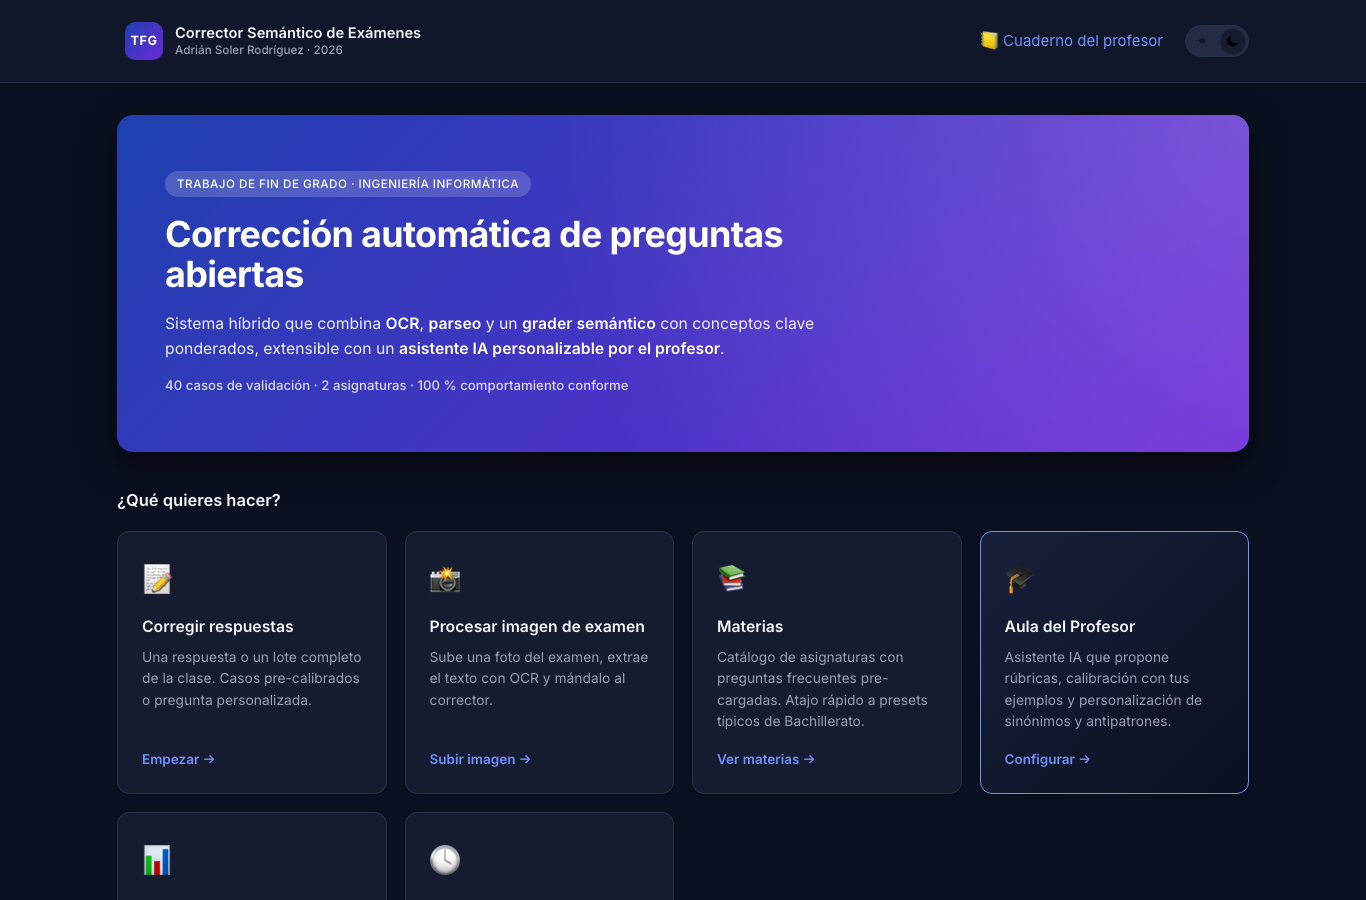
\includegraphics[width=0.85\textwidth]{web_landing.png}
\caption{Página de inicio de la aplicación web.}
\label{fig:web-landing}
\end{figure}

\begin{figure}[ht]
\centering
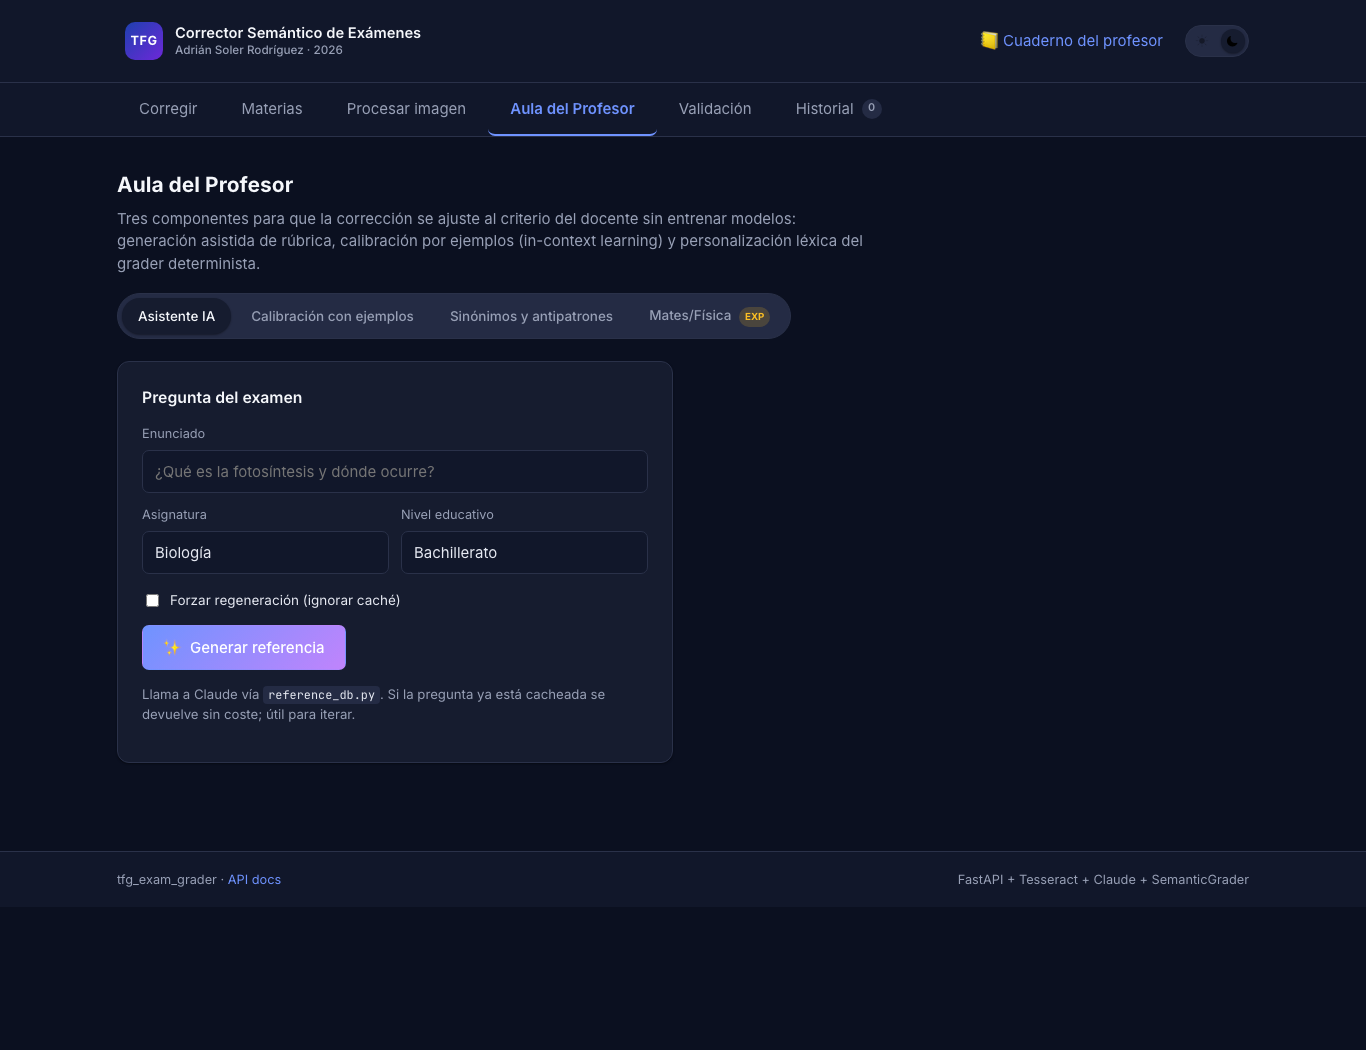
\includegraphics[width=0.92\textwidth]{web_aula.png}
\caption{``Aula del profesor'': asistente de rúbricas, calibración con ejemplos y gestión de sinónimos y antipatrones.}
\label{fig:web-aula}
\end{figure}

\begin{figure}[ht]
\centering
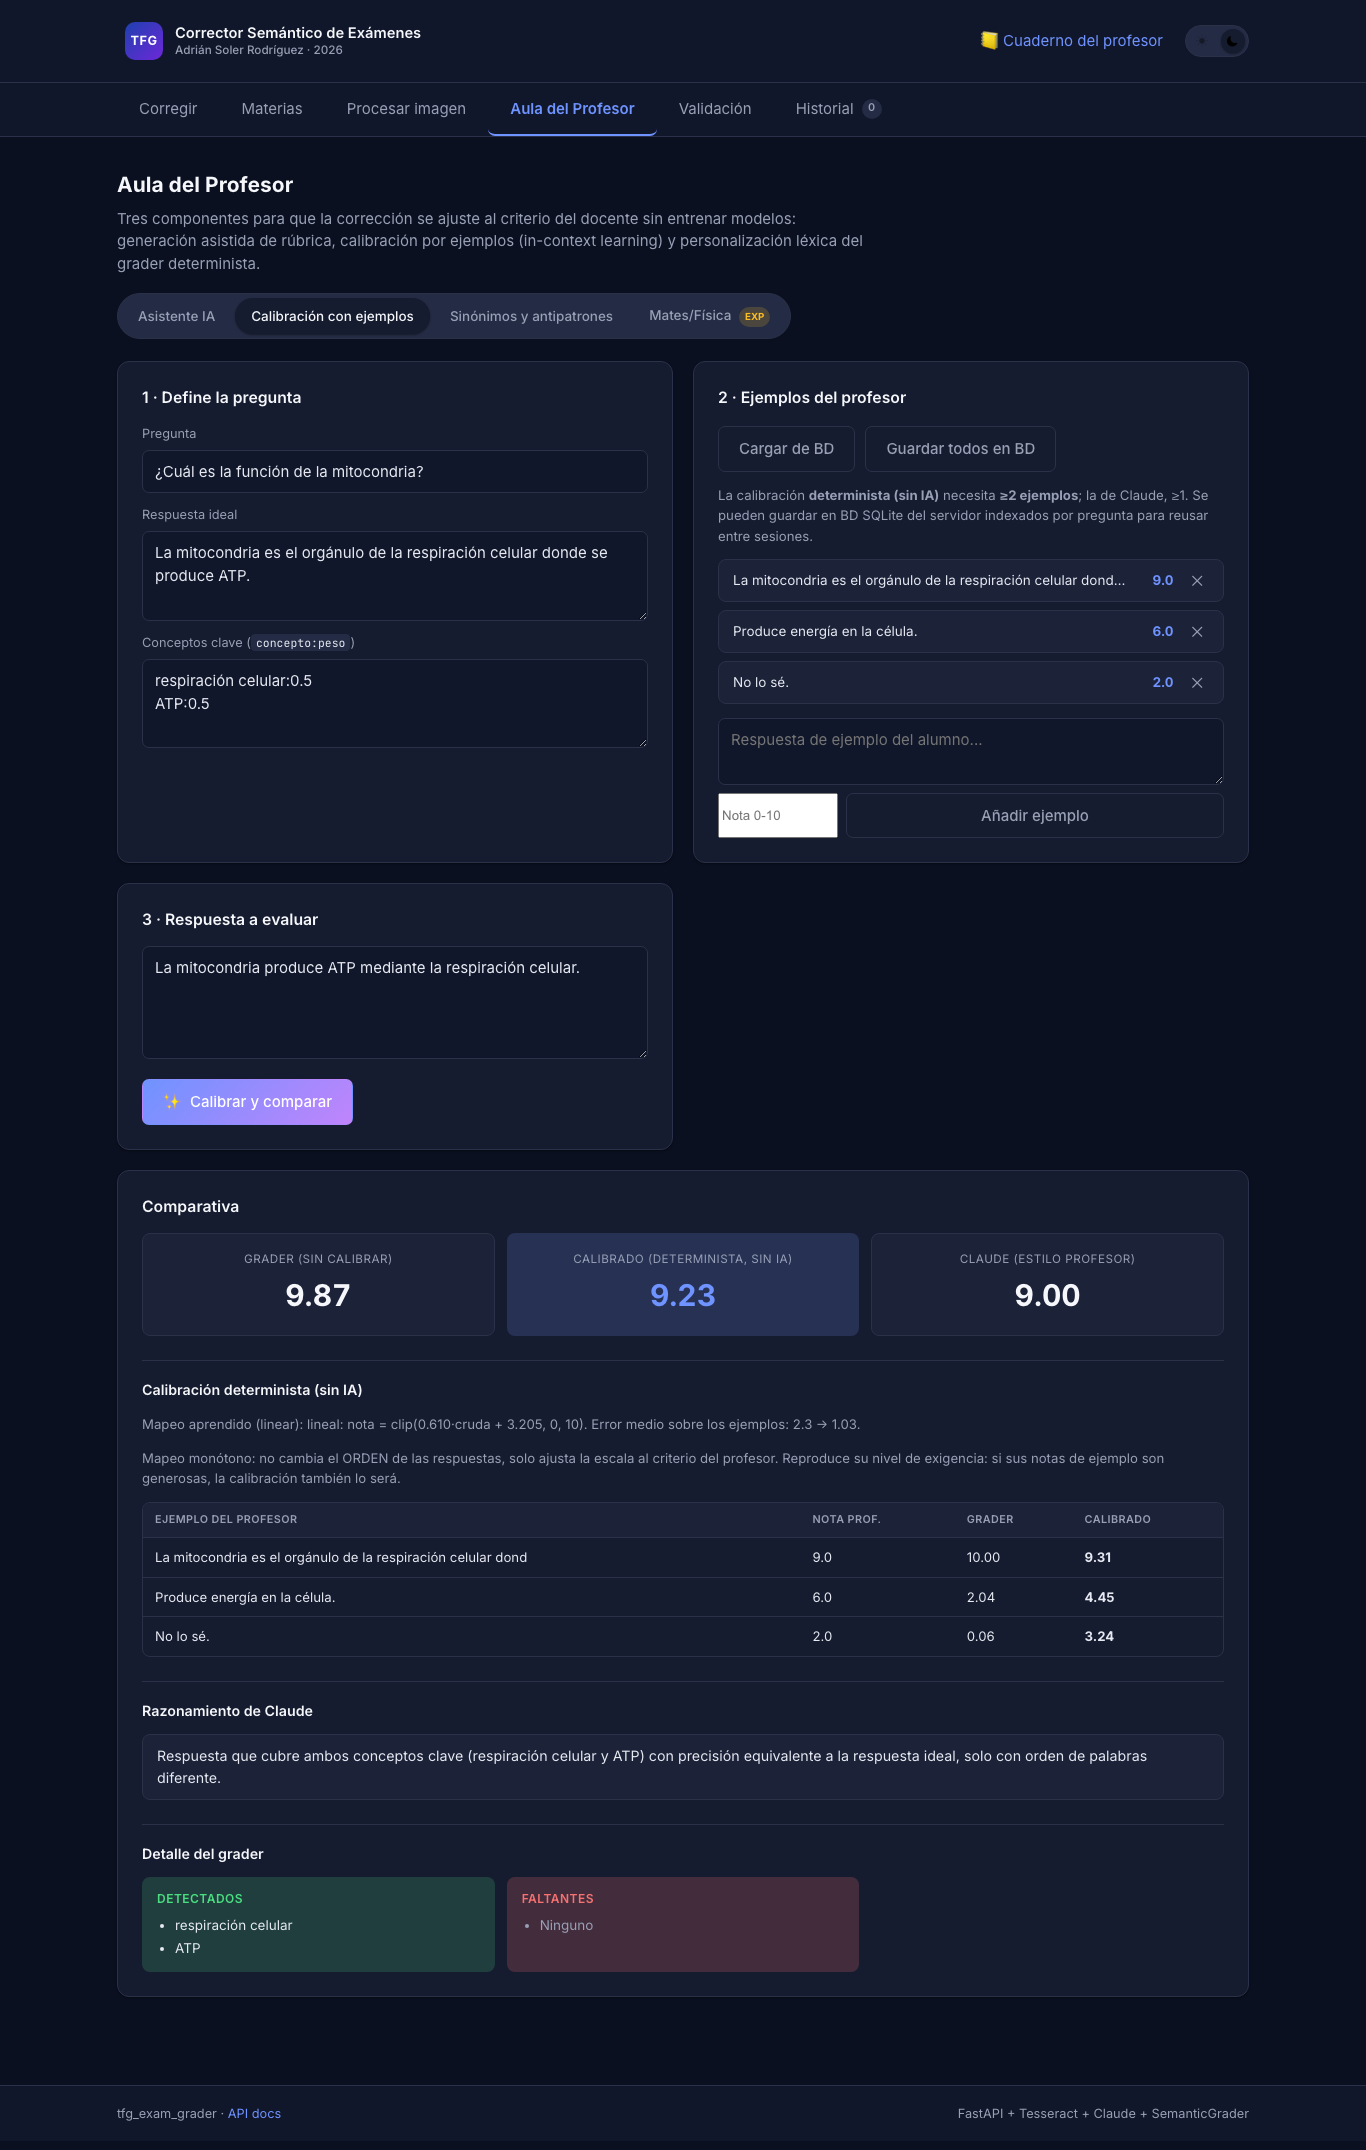
\includegraphics[width=0.7\textwidth]{web_calibracion.png}
\caption{Calibración con ejemplos. Para una nueva respuesta se comparan la nota cruda del grader (9{,}87), la calibrada de forma determinista (9{,}23) y la de Claude (9{,}00), junto al mapeo lineal aprendido y la tabla de ajuste sobre los ejemplos.}
\label{fig:web-calibracion}
\end{figure}

\cleardoublepage
\addcontentsline{toc}{chapter}{Referencias}
\bibliographystyle{apacite}
\bibliography{referencias}


\end{document}
